% =========================================================================
% EBB — AISTATS 2026 template version (migrated from the arXiv layout).
% Compile: pdflatex main.tex (x2).
% =========================================================================
\documentclass[twoside]{article}
\usepackage{aistats2026}

\usepackage{bold-extra}       % bold small caps for \EBB in bold headings
\usepackage{amsmath,amssymb,amsthm}
\usepackage{booktabs}
\usepackage{graphicx}
\usepackage[expansion=false]{microtype}
\usepackage[numbers,sort&compress]{natbib}
\usepackage{xcolor}
\usepackage[colorlinks=true,linkcolor=blue,citecolor=blue,urlcolor=blue]{hyperref}

\theoremstyle{definition}
\newtheorem{proposition}{Proposition}
\newtheorem{corollary}{Corollary}

\newcommand{\EBB}{\textsc{Ebb}}
\newcommand{\E}{\mathbb{E}}
\newcommand{\Var}{\mathrm{Var}}
\newcommand{\ind}[1]{\mathbf{1}\{#1\}}
\newcommand{\best}[1]{\textbf{#1}}
\newcommand{\secondbest}[1]{\underline{#1}}

\begin{document}

\runningtitle{When Does Pooling Pay? Forgetting, Credibility, and Intermittent Demand}
\runningauthor{Bai, Chu}

\twocolumn[
\aistatstitle{When Does Pooling Pay? A Credibility Diagnostic for\\
Forgetting and Pooling in Intermittent-Demand Forecasting}
\aistatsauthor{ Zong-Han Bai \And Po-Yen Chu }
\aistatsaddress{ } ]


% =========================================================================
% EBB v4 — Abstract / Introduction / Related Work
% Drop-in replacements. Macros, labels, and \citep keys unchanged.
% =========================================================================


% =========================================================================
% ABSTRACT  (replaces the existing abstract environment)
% =========================================================================
\begin{abstract}
Forecasting many sparse series forces two coupled choices: how much of
each series' own past to keep, and how much to borrow from other series.
We show that in a hierarchical empirical-Bayes hurdle model with one
exponential recency operator applied to item- and group-level statistics
alike, the two are one decision. Forgetting keeps a shared prior's
leverage alive while eroding the information that resolves fine group
structure; a two-sided credibility bound makes this precise, and its
resolution corollary turns it into a diagnostic computable from the
fitting window, before any pooling structure is fitted. On five public
intermittent-demand panels (more than 19{,}000 series), read against a
controlled surface over leverage and group separation, the diagnostic is
right in both directions. Where credibility is low the shared prior pays:
the advantage over a per-series Gaussian-process specialist grows from
two to three percent at full length to seven to eleven percent as
histories shrink. Where credibility is high, refining the partition is
worth nothing and nothing is found; on the one panel with room the
mixture objective fails to collect it, in data and in simulation alike.
The forecaster that carries the diagnostic, \EBB{}, selects pooling
structure, forgetting rate, and calibration layer on one validation tail,
and is, together with that specialist, the only method within five
percent of the best competitor on every panel under both fixed-origin and
strict walk-forward protocols, at one to three orders of magnitude lower
cost and with closed-form online updates. Two evaluation conventions
obscure such results: absolute-error metrics reward the all-zero forecast
on three panels, and static split-conformal wrappers understate what
conformal prediction achieves by about twenty percent.
\end{abstract}

\section{Introduction}\label{sec:intro}

Whether to fit each series on its own or to pool evidence across series
is the oldest question in forecasting many series at once, and the
working answer is still empirical: global models win on some collections
and lose on others, and one finds out by running both
\citep{monteromanso2021,januschowski2020,hewamalage2022}. The question is
sharpest for intermittent demand---long runs of zeros interrupted by
sporadic positive quantities, pervasive in spare parts, long-tail
commerce, and supply chains---because each series carries the least
evidence of its own. There, a second choice compounds the first. Old
observations can be discounted to track drift and obsolescence, but
forgetting also removes information. Local methods such as Croston, SBA,
and TSB \citep{croston1972,syntetos2005accuracy,teunter2011} adapt in
time while estimating each item separately; hierarchical probabilistic
models \citep{chapados2014,seeger2016,pitkin2024} shrink across items,
usually under a pooling structure and temporal model fixed in advance.
Pooling and forgetting are consequently designed as separate decisions.

They are not separate statistically. With exponential forgetting, an
item's effective history remains bounded, so a shared prior can retain
substantial influence even after a long observation sequence. The same
discounting, however, reduces the effective information used to estimate
each group-level prior. Stronger forgetting can therefore make pooling
more consequential while making fine pooling structure harder to resolve.
This tension is the paper's organizing principle: the forgetting rate
sets not only a temporal horizon but also the statistical resolution at
which cross-series structure can be learned, and both sides of the
trade-off are functions of one quantity---the credibility weight an item
retains after discounting---that can be computed from the fitting window
before any partition is fitted.

We develop this principle inside
\EBB{},\footnote{Empirical Bayes with Bounded memory: under the recency
operator an item's effective history stays bounded
(Section~\ref{sec:theory}), so evidence ebbs rather than accumulates.} a
recency-weighted hierarchical empirical-Bayes forecaster with
Beta--Binomial occurrence and log-normal size blocks represented by
per-item sufficient statistics. The same exponential weights enter the
item posterior and the group-level hyperparameters. A small candidate
family crosses discount factors with a global pool, the ADI/CV$^2$
taxonomy, and BIC-selected mixture partitions; one chronological
validation tail selects the discount, the structure, and, under
deployment, whether an adaptive conformal layer is applied. Estimation is
closed form apart from the mixture search, deterministic, and linear in
the number of observations.

The theory predicts an asymmetric pattern, and the experiments confirm
both halves of it. Where credibility is low the shared prior should
carry the forecast: truncating histories on five public panels, \EBB{}'s
advantage over the strongest per-series comparator, an official
Tweedie--Gaussian-process implementation, grows from two to three percent
at full length to seven to eleven percent with six months of history.
Where credibility is high, refining the pooling structure should be
worth little: a controlled surface that varies leverage and group
separation together places four panels where a supplied true partition
would earn nothing, and nothing is found; it places Carparts where one
would earn $1.7$ to $2.0\%$, and the learned partition returns $-0.08\%$
there, as the same objective does at those coordinates in simulation; a
screen built from the single-pool fit alone identifies, in simulation,
the regimes where refinement cannot pay materially. Forgetting itself is
a first-order decision: all five panels select it,
and where both effects are measurable it is worth an order of magnitude
more than refinement.

The forecaster is competitive on the terms that matter for deployment.
Across the five panels and both a fixed-origin and a strict walk-forward
protocol, \EBB{} and the Gaussian-process specialist are the only methods
within five percent of the best competitor everywhere; \EBB{} leads on
two panels, trails by under one percent on two, and by $2.9\%$ on M5 at
fixed origin, at one to three orders of magnitude lower cost and with
online updates that need no refitting.

\paragraph{Contributions.}
\textbf{(1) A two-sided resolution theory and an ex ante diagnostic.}
Proposition~\ref{prop:twosided} shows that one recency operator keeps
prior leverage active but raises the sampling-variance floor against
which group heterogeneity must be resolved; Corollary~\ref{cor:resolution}
converts this into a statistic computable from the fitting window that
bounds what any partition could be worth. A controlled surface over
leverage and separation calibrates the bound, a pre-fit screen built from
the single-pool fit identifies regimes without material room, and five
real panels confirm the diagnostic in both directions
(Section~\ref{sec:pays}).
\textbf{(2) A forecaster that carries the diagnostic.} \EBB{} selects
pooling structure, forgetting rate, and calibration layer on one
leakage-safe validation tail; its predictive law is closed form,
bit-reproducible, costs milliseconds per series, and updates online. It
matches a per-series Gaussian-process specialist to within a percent on
most panels and is the only other method within five percent of the best
competitor on all of them (Section~\ref{sec:accuracy}).
\textbf{(3) Two evaluation cautions.} Absolute-error metrics reward the
all-zero forecast on three of five panels and reverse the ranking of a
known-correct partition in simulation, and static split-conformal
wrappers understate what conformal prediction achieves by about twenty
percent relative to an adaptive construction
(Section~\ref{sec:cautions}). Comparators include the official TweedieGP
implementation, adaptive conformal inference applied to baselines and to
\EBB{} alike, a published hierarchical state-space model, and a zero-shot
foundation model.

\section{Related Work}\label{sec:related}

\textbf{Intermittent-demand forecasting.} Croston's decomposition
\citep{croston1972}, its SBA correction \citep{syntetos2005accuracy}, and
TSB \citep{teunter2011} estimate occurrence and positive size locally;
TSB additionally lets the occurrence estimate decay under obsolescence.
ADIDA \citep{nikolopoulos2011} and IMAPA \citep{kourentzes2016} instead
reduce intermittency through temporal aggregation, while likelihood-based
alternatives include inventory count models \citep{snyder2012}, iETS
\citep{svetunkov2023iets}, Tweedie Gaussian processes \citep{damato2025},
and deep renewal processes \citep{turkmen2019}. Conformal wrappers turn
point forecasters into predictive intervals, and adaptive conformal
inference updates miscoverage levels under distribution shift
\citep{gibbs2021}; we evaluate both the static and the adaptive form,
because the difference between them is larger than most method
differences reported on these panels. These approaches provide important
forms of temporal adaptation, but do not jointly learn how
recency-weighted evidence should be shared across items. Hierarchical
models do share evidence: \citet{chapados2014} and \citet{seeger2016}
pool related count series at scale, and \citet{pitkin2024} develops a
hierarchical hurdle model for retail. Their pooling structure or temporal
evolution is generally specified in advance. \EBB{} instead crosses
recency and pooling choices within one occurrence--size empirical-Bayes
model, and asks when that crossing can pay.

\textbf{Learning cross-series structure.} The continuum between local and
global forecasting is formalized by \citet{monteromanso2021}. More recent
work learns richer forms of cross-series specialization. For hierarchical
forecasting, \citet{cini2024} learns a graph-pooled aggregation hierarchy
aligned with the forecasting objective. Moirai-MoE \citep{liu2025moirai}
replaces human-defined frequency groups with token-level sparse-expert
routing in a time-series foundation model. These approaches motivate
data-adaptive structure, but address different objects: aggregation
coherence or latent expert specialization. Our groups are explicit
exchangeability pools for a shared prior. That restriction is what makes
their statistical resolution analyzable: the quantity governing whether a
pool can be estimated is the same credibility weight that governs whether
it can matter, so a single diagnostic covers both. It also permits a
direct comparison among global, fixed-rule demand-pattern, and learned
mixture pools under one predictive law.

\textbf{Discounting, credibility, and selection.} Exponential discounting
is classical in Bayesian dynamic models \citep{westharrison1997}, and
power priors down-weight historical likelihoods \citep{ibrahimchen2000}.
Likewise, $\lambda_i=n_i/(n_i+\phi_g)$ is the classical actuarial
credibility form \citep{buhlmann1967}; Proposition~\ref{prop:credibility}
is therefore a restatement, not a claimed contribution. The distinction in
\EBB{} is that one recency operator updates both item statistics and the
empirical-Bayes statistics defining the shared prior, and its strength is
selected jointly with the pool. Proposition~\ref{prop:twosided} then
identifies the resulting two-sided resolution limit: forgetting preserves
prior leverage but can erase the information needed to distinguish fine
pools. Chronological validation selects among the finite candidate family.
Because zero-heavy point losses can favor degenerate forecasts, selection
uses pinball loss, a proper scoring rule \citep{gneiting2007}, with the
high quantiles relevant to inventory decisions \citep{kolassa2016}.

% =========================================================================

\section{\EBB{}: Recency-Weighted Hierarchical EB}\label{sec:method}
% =========================================================================

\EBB{} combines two candidate choices inside one occurrence--size
model: a recency discount $w$ determines which observations remain
informative, and a partition $g$ determines which items share an
empirical-Bayes prior. The key construction is that the \emph{same}
discounted sufficient statistics determine both the item posterior and
the group prior. We first define that representation, then the candidate
partitions and their leakage-safe joint selection.

\subsection{Occurrence--size model}\label{sec:base}

For item $i$, let $z_{i,t}=\ind{y_{i,t}>0}$ and define
$\ell_{i,t}=\log y_{i,t}$ when $z_{i,t}=1$. Conditional on membership
$g_i=g(i)$, the hurdle model is
\begin{equation}
\begin{aligned}
\pi_i &\sim \mathrm{Beta}(\alpha_{g_i},\beta_{g_i}), &
z_{i,t}\mid\pi_i &\sim \mathrm{Bern}(\pi_i),\\
\mu_i &\sim \mathcal{N}(\mu_{0,g_i},\tau^2_{g_i}), &
\sigma_i^2 &\sim \mathrm{ScaleInv}\text{-}\chi^2(\nu,s^2_{0,g_i}),\\
\ell_{i,t} &\;\big|\; z_{i,t}{=}1,\mu_i,\sigma_i^2
\sim \mathcal{N}(\mu_i,\sigma_i^2).\span\span
\end{aligned}
\label{eq:model}
\end{equation}
Here $s^2_{0,g}$ is parameterized so that the prior mean of
$\sigma_i^2$ is the group estimate $\sigma_g^2$; $\nu$ is fixed rather
than selected. Group hyperparameters are estimated by empirical Bayes:
Beta--Binomial marginal likelihood for occurrence, and an
intercept-only random-effects fit plus conjugate variance shrinkage for
positive log-size. Appendix~\ref{app:implementation} gives the numerical
objectives and fallback rules.

Without forgetting, all inference depends on the four statistics
\[
S_i(1)=(n_i,c_i,u_i,v_i)
=\sum_{t=1}^{T_i}
  \bigl(1,z_{i,t},z_{i,t}\ell_{i,t},z_{i,t}\ell_{i,t}^2\bigr),
\]
where the last two terms are zero when $z_{i,t}=0$. The occurrence
posterior mean and the positive-size posterior location take parallel
credibility forms,
\begin{align}
\hat\pi_i
&=\lambda_i^{(o)}\bar p_i+(1-\lambda_i^{(o)})\mu_{\pi,g_i},
&\lambda_i^{(o)}&=\frac{n_i}{n_i+\phi_{g_i}},\nonumber\\
\hat\mu_i
&=\lambda_i^{(+)}\bar\ell_i+(1-\lambda_i^{(+)})\mu_{0,g_i},
&\lambda_i^{(+)}&=\frac{n_i^+}{n_i^++\kappa_{i,g_i}},
\label{eq:credibility-pair}
\end{align}
with $\phi_g=\alpha_g+\beta_g$ and
$\kappa_{i,g}=\hat\sigma_i^2/\tau_g^2$. Thus a partition matters only
through the prior target and strength supplied to its members.

Two variance ratios appear in what follows. Estimation uses the item-level
$\kappa_{i,g}=\hat\sigma_i^2/\tau_g^2$ in
\eqref{eq:credibility-pair}; the analysis in
Section~\ref{sec:resolution} works with the group-level surrogate
$\kappa_g=\sigma_g^2/\tau_g^2$, which replaces each item's process
variance by its group estimate. The two coincide when the group is
homogeneous in $\sigma_i^2$, and the surrogate is what the collapse event
of Proposition~\ref{prop:twosided} is stated in terms of.

The plug-in marginal predictive distribution is zero-inflated
log-normal:
\begin{equation}
\begin{aligned}
\Pr(Y_i=0\mid\mathcal D)&=1-\hat\pi_i,\\
\log Y_i\mid(Y_i>0,\mathcal D)
&\sim\mathcal N(\hat\mu_i,\hat\sigma_i^2+V_i),
\end{aligned}
\label{eq:predictive-law}
\end{equation}
where $V_i$ is posterior uncertainty in $\mu_i$. Its quantiles are
analytic. For point evaluation we retain the conditional plug-in mean
$\hat y_i=\hat\pi_i\exp(\hat\mu_i+\hat\sigma_i^2/2)$; it is distinct
from the mean of \eqref{eq:predictive-law}, which also integrates $V_i$.

\subsection{Shared recency weighting}\label{sec:discount}

For $w\in(0,1]$, replace $S_i(1)$ by
\begin{equation}
S_i(w)=\sum_{t=1}^{T_i}w^{T_i-t}
  \bigl(1,z_{i,t},z_{i,t}\ell_{i,t},z_{i,t}\ell_{i,t}^2\bigr).
\label{eq:discounted-stats}
\end{equation}
These fractional counts are valid weighted-likelihood statistics; the
log-Gamma form of the occurrence marginal and the Normal size objective
extend directly to them. Crucially, $S_i(w)$ is used twice:
\begin{equation}
\begin{aligned}
\widehat\eta_g(w)
&=\arg\max_{\eta_g}
  \sum_{i:g_i=g}\log m\{S_i(w)\mid\eta_g\},\\
q_i^{(w)}(\theta_i)
&=q_i\!\left(\theta_i\mid
  S_i(w),\widehat\eta_{g_i}(w)\right),
\end{aligned}
\label{eq:shared-recency}
\end{equation}
where $\eta_g$ collects the group hyperparameters and $q_i$ is the item
posterior. The group prior therefore adapts to recent cross-sectional
evidence rather than remaining a stationary prior applied to discounted
item data. Setting $w=1$ recovers the stationary estimator exactly.

For occurrence, \eqref{eq:credibility-pair} becomes
\begin{equation}
\begin{aligned}
\hat\pi_i(w)
&=\lambda_i(w)\bar p_i(w)
  +\{1-\lambda_i(w)\}\mu_{\pi,g_i}(w),\\
\lambda_i(w)
&=\frac{n_i(w)}{n_i(w)+\phi_{g_i}(w)}.
\end{aligned}
\label{eq:disc-post}
\end{equation}
The analogous positive-size update uses discounted positive mass
$n_i^+(w)$ and the group variance ratio $\kappa_{i,g}(w)$.


\subsection{Candidate pooling structures}\label{sec:mixture}

Let $\mathcal R$ contain three ways to construct $g(\cdot)$ from the
fitting data, ordered coarse to fine: a \emph{global} pool with one prior
for the panel; the \emph{taxonomy} of four ADI/CV$^2$ demand-pattern
classes at the classical thresholds \citep{syntetos2005categorization};
and a \emph{learned} partition, hard assignments from a mixture of
occurrence--size prior components with $K\in\{1,\dots,6\}$ selected by
BIC, fit by EM with an analytic responsibility update and a
deterministic initialization (Appendix~\ref{app:demoted},
Table~\ref{tab:pool-candidates}). The question this paper asks is not
which rung is best in general but whether the discounted data support
moving up the ladder at all; Section~\ref{sec:resolution} gives the
condition and Section~\ref{sec:pays} reports what happens when it fails.
Every data-dependent label is computed from the selector's fitting head,
never its validation tail.

\subsection{Leakage-safe joint selection}\label{sec:select}

Each training series is split chronologically into a fitting head
$\mathcal H_i$ (first $80\%$) and validation tail $\mathcal V_i$ (last
$20\%$). For every $(r,w)\in\mathcal R\times\mathcal W$, with
\[
\mathcal W=\{1,.999,.997,.995,.99,.98,.95,.90\},
\]
the partition builder for $r$ sees only $\mathcal H=\cup_i\mathcal H_i$.
The resulting labels, discounted EB prior, and item posteriors are all
fit on the same head. The candidate is scored by
\begin{equation}
\begin{aligned}
\widehat R(r,w)
&=\frac{1}{N_{\!V}}\sum_{i\in\mathcal I_V}
  \frac{1}{|\mathcal V_i||\mathcal Q|}\\[-0.25em]
&\quad\times
  \sum_{t\in\mathcal V_i}\sum_{q\in\mathcal Q}
  \frac{\rho_q(y_{i,t},\widehat Q_{i,t}^{(r,w)}(q))}{a_i},
\end{aligned}
\label{eq:selection-risk}
\end{equation}
where $\mathcal Q=\{.5,.75,.9\}$, $\rho_q$ is pinball loss, and $a_i$
is mean absolute demand on the fitting head (with a panel-level fallback
for an all-zero head); $N_V=|\mathcal I_V|$ is the number of scored
items. Times and quantiles are averaged within item
before items receive uniform weight. This matches the panel-level goal
and prevents long series or high-volume items from dominating selection.

The selected pair is
$(\hat r,\hat w)=\arg\min_{r,w}\widehat R(r,w)$. Its partition is then
\emph{relearned} on the complete training window at $\hat w$, and the EB
model is refit once before external evaluation. Thus the validation tail
chooses a construction rule and discount, not a permanent set of labels;
external targets are never used. There are 24 outer forecast candidates.

\paragraph{Resolution diagnostics.} Fitting each candidate already
produces everything the resolution analysis of Section~\ref{sec:resolution}
needs: for every $(r,w)$ and group $g$ the selector records, from the fitting
head only, the median credibility weights $\lambda_i^{(o)}$ and
$\lambda_i^{(+)}$, the share of items with $\lambda_i^{(+)}<0.1$, the group
sizes, and the resolution statistic $\hat z_g$ whose nonpositive values
coincide with the collapse event of Proposition~\ref{prop:twosided}
(Appendix~\ref{app:demoted}). They are computed before any external
observation is seen, and Section~\ref{sec:pays} reads them.

Appendix~\ref{app:implementation} gives split edge cases and
pseudocode-level implementation details.


\subsection{Forecasts and computation}\label{sec:complexity}

Selection uses the analytic plug-in quantiles in
\eqref{eq:predictive-law}. The reported probabilistic forecasts also
average quantile estimates across $B=20$ cross-item bootstrap refits of
the group hyperparameters. We treat this explicitly as a quantile
ensemble; the average of component quantiles is not asserted to be the
quantile of a single posterior mixture.

For each $w$, one pass computes $S_i(w)$ in $O(\sum_iT_i)$ time. Each EB
fit requires only low-dimensional deterministic optimization per group;
mixture EM is $O(NK)$ per iteration. Prediction is $O(N)$ for points and
$O(NQ)$ for $Q$ quantiles.

\section{Resolution under Forgetting}\label{sec:theory}
% =========================================================================

The shared operator in \eqref{eq:shared-recency} creates two opposing
effects. A bounded item history prevents the group prior from vanishing,
but the same bound limits the information used to estimate fine group
structure. This section formalizes that interaction. Supporting results
connecting the model to TSB, drift tracking, finite-class selection, and
classical credibility are collected in Appendix~\ref{app:supporting}.

\subsection{Persistent prior leverage}

Fix an item and suppress its subscripts. Because
$n(w)=\sum_{t=1}^{T}w^{T-t}\le(1-w)^{-1}$ for $w<1$, the occurrence
credibility weight cannot converge to one: $\lambda(w)\le\{1+(1-w)\phi\}^{-1}<1$
for every horizon, whereas $\lambda(1)\to1$ as $T\to\infty$
(Proposition~\ref{prop:active}, Appendix~\ref{app:demoted}). Forgetting
keeps the pooled prior relevant indefinitely; the statement is about
leverage, not benefit.

\subsection{Variance-component resolution}\label{sec:resolution}

The converse problem appears in the positive-size block. Let item $i$
in group $g$ have discounted positive mass $n_i^+$, sampling variance
$s_i=\sigma_g^2/n_i^+$ for its log-size mean, and credibility
$\lambda_i^{(+)}=n_i^+/(n_i^++\kappa_g)$ with
$\kappa_g=\sigma_g^2/\tau_g^2$. The group variance is estimated by the
truncated moment/REML form
$\hat\tau_g^2=\max(0,S_g^2-\bar s_g)$, where $S_g^2$ is the sample
variance of the $m_g$ item means and
$\bar s_g=m_g^{-1}\sum_{i\in g}s_i$.

\begin{proposition}[Two-sided effect of forgetting]
\label{prop:twosided}
\textbf{(i)} For $w<1$,
$\lambda_i^{(+)}\le\{1+(1-w)\kappa_g\}^{-1}<1$.
\textbf{(ii)} For independent item means with possibly unequal $s_i$,
\[
\E[S_g^2]=\tau_g^2+\bar s_g
\]
holds exactly. Under the Gaussian moment approximation,
\begin{equation}
\Pr(\hat\tau_g^2=0)\simeq
\Phi\!\left(-\sqrt{\frac{m_g-1}{2}}\,\rho_g\right),
\qquad
\rho_g=\frac{\tau_g^2}{\tau_g^2+\bar s_g}.
\label{eq:collapse-prob}
\end{equation}
Since $n_i^+\le(1-w)^{-1}$,
$\bar s_g\ge(1-w)\sigma_g^2$ and therefore
\[
\rho_g\le
\frac{\tau_g^2}{\tau_g^2+(1-w)\sigma_g^2}.
\]
On the collapse event the plug-in estimate has $\hat\tau_g^2=0$ and
$\lambda_i^{(+)}=0$: the item mean is replaced by its estimated group
mean.
\end{proposition}

The population ratio $\rho_g$ is not observed. For diagnostics we use
\[
\hat z_g=\frac{S_g^2-\bar s_g}
{\sqrt{2/(m_g-1)}\,S_g^2},
\]
whose nonpositive values coincide with the plug-in collapse event.

\begin{corollary}[Resolution condition]
\label{cor:resolution}
For this estimator and window, stable estimation of a group variance
requires, up to a fixed probability threshold,
\begin{gather*}
\rho_g\sqrt{m_g-1}\gtrsim1,\\
\text{equivalently}\qquad
\tau_g^2\gtrsim
\frac{\bar s_g}{\sqrt{m_g-1}-1},
\end{gather*}
with $\bar s_g\ge(1-w)\sigma_g^2$.
\end{corollary}

For similarity-based refinements, finer groups typically reduce both
$m_g$ and the within-group spread $\tau_g^2$, while stronger forgetting
raises the sampling-variance floor. All three changes move the estimator
toward collapse. This is an estimator- and window-specific resolution
condition, not an information-theoretic lower bound, and it does not say
which candidate wins below the threshold.

\begin{figure*}[!t]
\centering
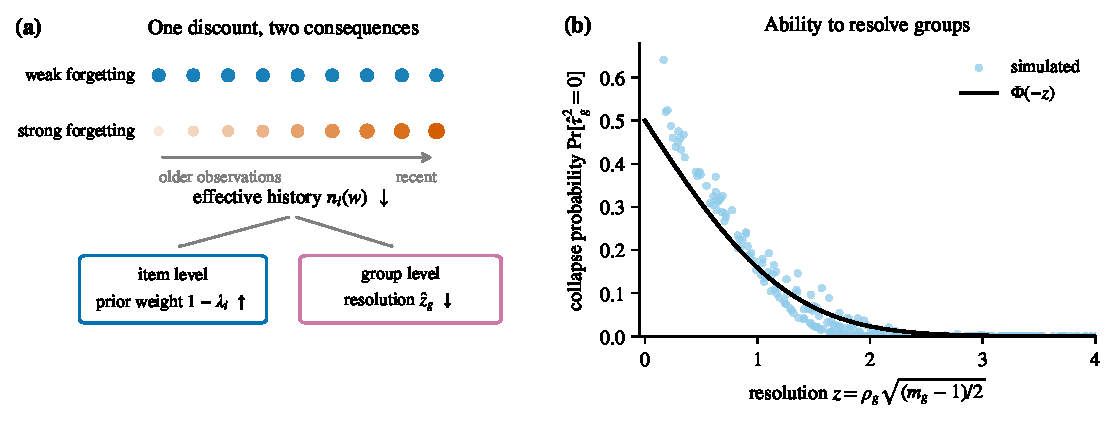
\includegraphics[width=0.92\textwidth]{fig01_mechanism_v2.pdf}
\caption{\textbf{One discount creates two opposing effects.}
\textbf{(a)} The same recency operator reduces item effective history,
which increases prior leverage, and group effective information, which
reduces structural resolution. \textbf{(b)} When the partition must be
estimated, the probability that
the group variance collapses rises as the resolution statistic falls;
the curve is the approximation in \eqref{eq:collapse-prob}.}
\label{fig:mechanism}
\end{figure*}

Figure~\ref{fig:mechanism} summarizes why pooling can become more
consequential at exactly the point where a fine partition becomes harder
to estimate. Section~\ref{sec:synthetic} tests both sides with known group
labels. Proofs and the accuracy limits of the approximation are given in
Appendix~\ref{app:proofs} and Section~\ref{sec:limitations}.
% =========================================================================
% EBB v6 — sections/experiments_v6.tex (assembled by scripts/integrity/v6_build.py)
% =========================================================================
\section{Experiments}\label{sec:experiments}

\subsection{Experimental design}\label{sec:setup}

\textbf{Datasets.} We evaluate on two daily panels---\textbf{Online
Retail} \citep{chen2015} (3{,}649 series) and a seed-controlled
5{,}000-series \textbf{M5} sample \citep{makridakis2022}---and the
monthly intermittent suite of \citet{damato2025}: \textbf{Auto}
(3{,}000 series), \textbf{Carparts} (2{,}509), and \textbf{RAF}
(5{,}000). Together they contain more than 19{,}000 series and span
long daily histories and short, highly sparse monthly panels. Dataset
construction and holdout lengths are in Appendix~\ref{app:datasets}.
Both the probabilistic and the point M5 protocols use the first two
thirds of each series for initialization.

\textbf{Comparators.} The classical set comprises Croston, SBA, TSB,
ADIDA, and IMAPA; stronger statistical comparators are AutoARIMA,
AutoTheta, a per-series autoregressive Tweedie GLM, iETS, and the official
TweedieGP implementation at its released defaults on all five panels.
For probabilistic
evaluation we use native distributions where available and chronological
split-conformal wrappers (CP-$\ast$) for the point forecasters. The
walk-forward studies additionally include adaptive conformal inference
(ACI) applied to ADIDA and to \EBB{} on every panel and to TSB on Online
Retail; ACI-\EBB{} reads \EBB{}'s analytic predictive quantile at the
adaptive level, with the same $\gamma$ and update rule as ACI-ADIDA;
\EBB{} (rule) applies that layer only where a validation-tail rule inside
the initialization window selects it (Section~\ref{sec:walkforward}). A 25-candidate tuned-TSB control
receives the same internal chronological selection budget as \EBB{}.
DeepState and Chronos-Bolt comparisons are confined to
Appendix~\ref{app:neural} because they use subset or proxy protocols.
Implementation details and complete settings are in
Appendix~\ref{app:implementation}.

\textbf{Protocols and metrics.} The primary fixed-origin experiment fits
once on the initialization window and scores the full evaluation span.
A strict walk-forward experiment then reveals and updates one block at a
time: seven-day blocks on Online Retail and M5, one-month blocks on Auto,
Carparts, and RAF. Classical, conformal, and TweedieGP methods refit each
block, except that on Online Retail AutoARIMA, AutoTheta, iETS, and
TweedieGP refit every four blocks and on M5 only the conformal and
adaptive-conformal wrappers are run (Appendix~\ref{app:efficiency} gives
the cost of the rest); \EBB{} updates discounted sufficient statistics
each block. The primary metric is
scaled pinball loss (SPL; lower is better), averaged over
$q\in\{0.1,0.25,0.5,0.75,0.9\}$; we separately report q90 and the far tail
because inventory decisions are asymmetric. All quantiles are
zero-truncated and monotonized, and \EBB{} is reported without post-hoc
calibration. Every model in Table~\ref{tab:prob} is scored by one
implementation from its stored quantile predictions, so no cell mixes
scoring versions. Fixed-origin, walk-forward, and subset foundation model
results are kept separate because they answer different questions. MAE and
RMSSE are secondary diagnostics rather than the headline criteria because
zero forecasts can minimize absolute error on intermittent panels. Full
point, interval, significance, and efficiency results are in
Appendix~\ref{app:extra}.

% =========================================================================


% =========================================================================
\subsection{Where pooling pays}\label{sec:pays}
% =========================================================================

The diagnostic of Section~\ref{sec:resolution} makes two predictions:
that a shared prior's return grows as an item's own credibility falls, and
that refining the pooling structure returns something only where the
discounted data both leave room and resolve the structure. We test each
side on the five panels, using the credibility weights at the audited
configurations (Appendix~\ref{app:demoted}, Table~\ref{tab:leverage})
and a controlled study that varies leverage and group separation together
(Appendix~\ref{app:demoted}, Table~\ref{tab:sanity};
Appendix~\ref{app:simulation-details}).

\paragraph{Short histories: the shared prior pays.}
Corollary~\ref{cor:resolution} predicts where a pooled prior pays: when an
item's own evidence is thin, its credibility weight is low and the shared
prior carries the forecast. Truncating the initialization window to its
last $L$ observations per series, with the evaluation span unchanged,
moves every panel along that axis. Figure~\ref{fig:coldstart} plots
\EBB{}'s mean-SPL advantage over TweedieGP, the strongest per-series
comparator, against the retained history; Table~\ref{tab:coldstart} gives
the numbers together with the median credibility weights and the static
conformal wrapper. The advantage grows as history shrinks on Auto and RAF,
turns positive on Carparts only at the shortest window, stays within a
third of a percent on Online Retail, and does not appear on M5, where both
median credibility weights stay above $0.8$ even with 28 days of history
and the per-series GP leads at every length but one, by a margin that
grows with the history it is given.
Both methods degrade gracefully; the gap that opens at short histories is
the pooled prior's contribution, and its size tracks the leverage the
diagnostic assigns to each panel rather than the panel's frequency.

\begin{figure}[t]
\centering
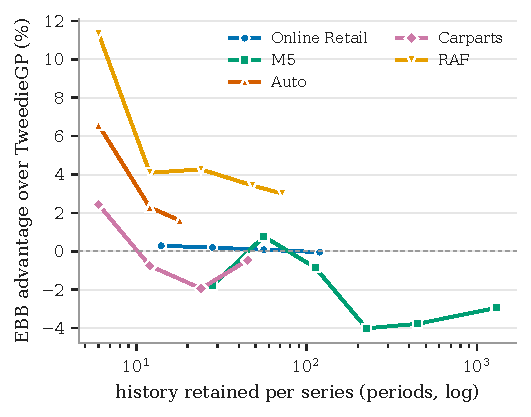
\includegraphics[width=0.98\linewidth]{figs/fig13_coldstart.pdf}
\caption{\textbf{Pooling pays when histories are short.} \EBB{}'s
mean-SPL advantage over TweedieGP (percent) against the history retained
per series at initialization; the evaluation span is fixed and the audited
structure and discount are unchanged. Full-length points reproduce
Table~\ref{tab:prob}.}
\label{fig:coldstart}
\end{figure}

\begin{figure*}[t]
\centering
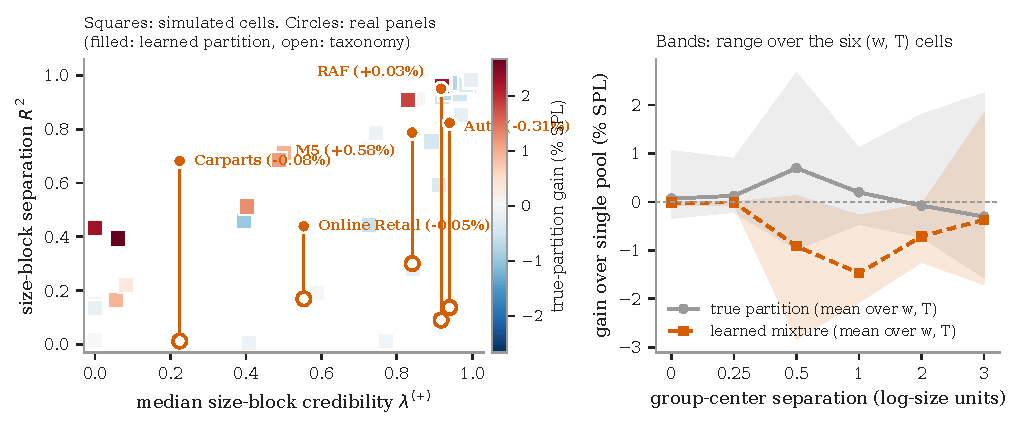
\includegraphics[width=0.98\textwidth]{figs/fig14_separation_surface.pdf}
\caption{\textbf{Room depends on separation as well as leverage, and the
real panels have little of it.} Left: each square is one cell of the
controlled grid (separation $\times$ discount $\times$ length, nine paired
replicates; occurrence separation scaled with size separation), placed at its median size-block credibility and at the share
of item log-size variance its true partition explains ($R^2$), colored by
the true partition's SPL gain over a single pool. Real panels are placed
at the same two coordinates, with $R^2$ measured under the learned
partition (filled) and under the objective-free ADI/CV$^2$ taxonomy (open);
labels give the learned partition's realized refinement gain. Right: the
true partition's gain and the learned mixture's gain against separation,
averaged over the six $(w,T)$ cells, with the range across cells shaded.
Room read within each panel's own forgetting regime is in
Table~\ref{tab:separation}.}
\label{fig:separation}
\end{figure*}

\paragraph{Where the room is, and whether it is collected.}
Figure~\ref{fig:separation} places the five panels on a surface that
varies leverage and group separation together. Each panel's size-block
separation is measured as the share of item log-size variance explained
by a partition, $R^2$, under its learned partition ($0.44$ to $0.95$) and
under the objective-free ADI/CV$^2$ taxonomy ($0.01$ to $0.30$); the
simulated cells carry the same statistic under their true labels. Read
within each panel's own forgetting regime (Table~\ref{tab:separation}), a
supplied true partition would earn between $-0.5\%$ and $+0.6\%$ on
Online Retail, M5, Auto, and RAF, and $1.7$ to $2.0\%$ on Carparts. The
learned partitions return $-0.05\%$, $+0.58\%$, $-0.31\%$, $+0.03\%$, and
$-0.08\%$: within the surface's range on the four panels without room,
and about two points short on the one panel with it. At Carparts's
coordinates the simulated learned mixture also loses ($-0.7\%$ to $-0.8\%$), and across the grid it is negative at every moderate
separation (Figure~\ref{fig:separation}, right), recovering the true
partition's return only when centers are two or more log-units apart and
histories are long. The earlier reading of Online Retail as the decisive
case rested on an envelope that pooled separations; resolved, its room is
at most $0.6\%$.

This separates the two explanations that aggregate results cannot. On
four panels the credibility weights and the separation together say there
is little to exploit, and the estimator's near-zero refinement gains are
the predicted outcome, not a failure. On Carparts the structure would pay
and the objective does not find it; that the same objective fails on
simulated panels at the same coordinates makes learnability, not the
bound, the binding constraint there. Corollary~\ref{cor:resolution}
bounds the prize; the surface says where the prize is nonzero.

\paragraph{Forgetting is an order of magnitude larger.}
Computed within a single selection surface under one definition---the
M5 surface at its selected discount---refining the pooling
structure is worth $+0.58\%$ of validation SPL, while discounting at the
same structure is worth $8.95\%$ for the global pool and $9.46\%$ for the
mixture. The asymmetry that motivates the paper survives at an order of
magnitude, and it survives on the one panel where refinement is
measurable at all.


\paragraph{A pre-fit screen.}
The surface answers the question ex post, with true labels; the
practical question is ex ante. On an expanded controlled grid
(separation, discount, length, occurrence rate, group size, imbalance;
$2{,}700$ panels), a closed-form score computed from the single-pool fit
alone, $\mathrm{med}_i(1-\lambda_i^{(+)})^2\,\hat\tau^2$, ranks the room a
true partition could earn with held-out AUC 0.71--0.71 for
the event ``gain above one percent''; a logistic screen on the same
fitting-window quantities reaches 0.84--0.83 when separation
levels, lengths, or random folds are held out and 0.68 when a
whole discount is held out, so the screen interpolates across regimes it
has seen and does not extrapolate across the discount
(Appendix~\ref{app:room}). Two facts bound the claim. 39\% of the
simulated single-pool fits collapse ($\hat\tau^2=0$) and half of the
large oracle gains occur there: escapes from a collapsed global fit,
which the resolution statistic flags, not returns to structure. And on
real series with a known partition injected---group offsets of up to two
log-units on Online Retail, Carparts, and M5, at the selected discount and
at $w=0.90$---the oracle partition never earns more than 0.4\%,
because a single pool absorbs the injected heterogeneity into
$\hat\tau^2$ and the items' own evidence takes over; the screen assigns
every such panel a probability below 0.17 of material room,
correctly, but the test checks rejections, not detections. The screen
therefore does what Corollary~\ref{cor:resolution} licenses and no more:
it identifies, from the fitting window, regimes where refinement cannot
pay materially.


% =========================================================================
\subsection{Accuracy and cost}\label{sec:accuracy}
% =========================================================================

\begin{table*}[t]
\centering
\caption{\textbf{Mean scaled pinball loss on five panels under two
protocols.} Fixed origin fits once and scores the full evaluation span;
walk-forward reveals one block at a time (seven days on the daily panels,
one month on the monthly ones), with every baseline refit per block and
\EBB{} updating sufficient statistics. The first row is the best of ten
classical, automatic, and static split-conformal baselines in each cell
(Online Retail: iETS / AutoTheta; M5: CP-Croston / CP-IMAPA; Auto: AutoARIMA / AutoARIMA; Carparts: CP-IMAPA / CP-IMAPA; RAF: CP-ADIDA / CP-ADIDA).
ACI-ADIDA is adaptive conformal inference on ADIDA; \EBB{} (rule) applies
the same adaptive layer to \EBB{} only where a validation-tail rule inside
the initialization window selects it, and is not ranked. Bold marks the
column's best ranked method. Full tables with all quantiles, coverage,
significance, and cost are in Appendix~\ref{app:demoted} and
Appendix~\ref{app:extra}.}
\label{tab:main}
\small
\setlength{\tabcolsep}{3.6pt}
\begin{tabular}{lrrrrrrrrrr}
\toprule
 & \multicolumn{5}{c}{Fixed origin} & \multicolumn{5}{c}{Walk-forward}\\
\cmidrule(lr){2-6}\cmidrule(lr){7-11}
Method & OR & M5 & Auto & Carp. & RAF & OR & M5 & Auto & Carp. & RAF\\
\midrule
Best classical or static-conformal baseline & 0.985 & 1.690 & 0.319 & 0.356 & 0.310 & 1.059 & 1.546 & 0.314 & 0.349 & 0.309\\
ACI-ADIDA & --- & --- & --- & --- & --- & 0.911 & \best{1.419} & 0.315 & 0.342 & 0.308\\
TweedieGP (per-series GP) & \best{0.884} & \best{1.623} & 0.298 & \best{0.321} & 0.276 & \best{0.853} & --- & 0.292 & \best{0.312} & 0.280\\
\midrule
\EBB{} & 0.885 & 1.671 & \best{0.294} & 0.323 & \best{0.268} & 0.854 & 1.485 & \best{0.291} & 0.315 & \best{0.268}\\
\EBB{} (calibration by rule) & --- & --- & --- & --- & --- & 0.854 & 1.379 & 0.290 & 0.315 & 0.268\\
\bottomrule
\end{tabular}
\end{table*}

Table~\ref{tab:main} reports the comparison that a practitioner would
make. At fixed origin, \EBB{} attains the lowest mean SPL on Auto and RAF,
by $1.6\%$ and $3.0\%$ over the official TweedieGP implementation, both
significant; TweedieGP attains it on Online Retail, Carparts, and M5, by
$0.05\%$, $0.5\%$, and $2.9\%$, of which only the M5 margin is
significant. Against every other comparator \EBB{} is best on all five
panels, by $10.1\%$ over iETS on Online Retail and $1.2\%$ over
CP-Croston on M5 (Appendix~\ref{app:demoted}, Table~\ref{tab:prob};
significance in Appendix~\ref{app:extra}, Table~\ref{tab:spl-significance}).
Under strict walk-forward updating the picture repeats for the
uncalibrated methods: \EBB{} leads on Auto and RAF, TweedieGP on Online
Retail and Carparts by $0.2\%$ and $0.8\%$, and per-series paired tests
cannot separate the two on three of the four panels where both run.
Adaptive conformal inference on ADIDA leads M5 by $4.4\%$; the same layer
applied to \EBB{} lowers its M5 loss from $1.485$ to $1.379$, $2.9\%$
below ACI-ADIDA, but degrades Online Retail and RAF, so whether to apply
it is itself selected on the validation tail. The rule applies the layer
on M5 and Auto, withholds it elsewhere, matches the ex-post better variant
on four of five panels, and leaves \EBB{} (rule) within $0.8\%$ of the
best competing method on every panel (Appendix~\ref{app:demoted},
Tables~\ref{tab:wfprob}--\ref{tab:regret}; Appendix~\ref{app:extra},
Table~\ref{tab:aci-rule}).


\begin{figure}[t]
\centering
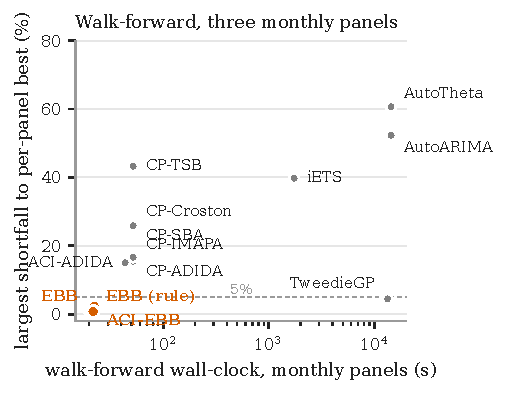
\includegraphics[width=0.98\linewidth]{figs/fig12b_frontier_wf.pdf}
\caption{\textbf{Largest shortfall against cost under walk-forward
updating.} Each point is one method on the three monthly panels, on which
every method has a measured wall-clock: $y$ is its largest mean-SPL
shortfall to the per-panel best, $x$ the total walk-forward wall-clock
(TweedieGP uses twelve workers, every other method one process). The
fixed-origin counterpart and the full regret tables are in
Appendix~\ref{app:demoted}.}
\label{fig:frontier}
\end{figure}

Figure~\ref{fig:frontier} summarizes both protocols by the largest
shortfall to the per-panel best against measured cost. \EBB{} and
TweedieGP are the only methods within five percent of the best competitor
everywhere (\EBB{} at most $3.0\%$ at fixed origin and $4.6\%$ under
walk-forward updating; TweedieGP $3.1\%$ and $4.5\%$); every other method
is at least $15\%$ behind on some panel. The two differ in cost by one to
three orders of magnitude: TweedieGP refits per-series variational GPs at
every update, so its walk-forward runs took between $36$ minutes and
$2.4$ hours with twelve workers and project to about $51$ hours on M5,
whereas \EBB{} completes each of the five walk-forward runs in under $40$
seconds on one core, updating sufficient statistics in closed form
(Appendix~\ref{app:efficiency}). Point forecasts are competitive but not
uniformly best (Appendix~\ref{app:point}).

% =========================================================================
\subsection{Two evaluation cautions}\label{sec:cautions}
% =========================================================================

The first caution concerns the probabilistic baseline: \emph{the choice of conformal construction matters more here than
the choice of forecaster}: making the wrapper adaptive
\citep{gibbs2021} improves ADIDA's mean SPL from $1.1576$ to $0.9108$, a
$21\%$ gain that is more than three times the remaining gap to \EBB{}.
Static split-conformal wrappers are the standard probabilistic baseline in
this literature; on this evidence they understate what conformal
prediction can do on intermittent panels, and comparisons drawn against
them---including earlier versions of our own---are correspondingly
generous.
The second caution concerns point metrics. The all-zero forecast attains
the lowest MAE on three of five panels and, in the controlled study, a
known-correct partition is reported as harmful by MAE while improving
every proper scoring rule (Appendix~\ref{app:demoted},
Table~\ref{tab:sanity}); absolute-error criteria should not be the sole
basis for comparing intermittent-demand forecasters, and we use them
only as diagnostics.


\section{Limitations}\label{sec:limitations}

\textbf{(1) The remaining gap to a per-series specialist.} The
log-normal size block keeps item posteriors analytic, and official
TweedieGP is better on Online Retail, Carparts, and M5 at fixed origin
and on Online Retail and Carparts under walk-forward updating, by under
one percent except on M5 ($2.9\%$). Three model-side remedies were tested
and none closes it (Appendix~\ref{app:negative}): heavier-tailed size
laws move mean SPL by at most $0.003$, item-specific forgetting rates
improve M5 by $1.2\%$ but leave it $1.8\%$ behind, and a separate
occurrence discount moves M5 by $0.14\%$. The gap lies in the posterior,
where the specialist adapts each series in time with one latent process
for occurrence and size, not in the predictive law's shape or the
forgetting schedule.

\textbf{(2) What the resolution condition is, and what it is not.}
Corollary~\ref{cor:resolution} uses a Gaussian working model and a
$\chi^2$ approximation, accurate except for small groups with strongly
unequal counts, where it understates the collapse probability by up to
$0.21$; it is an estimator-specific estimability statement, not an
information-theoretic bound. Its calibration on the controlled surface
is simulation-based, and the room it assigns to a real panel is read
within the panel's forgetting regime with an interpolation across two
series lengths. The pre-fit screen interpolates across regimes it has
seen and does not extrapolate across the discount, and its real-series
transfer test could check only rejections, since an injected partition
never earns material room once a single pool has absorbed the
heterogeneity. On the one panel with room, Carparts, neither the real
nor the simulated learned partition collects it, and neither label
sample-splitting nor credibility shrinkage of the group variance recovers
the loss in simulation (Appendix~\ref{app:simulation-details}); a
partition objective that maximizes resolvable separation rather than
marginal likelihood is the implicated next step.

\textbf{(3) Scope.} We do not run the external hierarchical Bayesian
implementations we cite; a same-model Gibbs sampler matches plug-in EB
within $0.1\%$ (Appendix~\ref{app:mcmc}), so the inference half of that
gap is closed and the model-class half is not. The adaptive conformal
comparison is one ACI design; given how much it moves the baseline, the
remaining designs deserve more attention. Selection uses one pinball
score; the discount selected at fixed origin is reused under walk-forward
updating without re-selection; DeepState, Chronos-Bolt, and Deep Renewal
Process comparisons use subset or proxy protocols
(Appendix~\ref{app:neural}); CRPS and a cost-based criterion remain
unrun.

\section{Conclusion}\label{sec:conclusion}

Forgetting and pooling are one decision. In a hierarchical
empirical-Bayes hurdle model with a single recency operator, the
credibility weight an item retains after discounting governs both how
much a shared prior can move its forecast and how well the data can
resolve the structure of that prior; a two-sided bound makes the
trade-off explicit and its corollary makes it computable before a
partition is fitted. On five public panels the diagnostic is right in
both directions. Where credibility is low the shared prior pays, and it
pays more the shorter the histories become. Where it is high, refining
the pooling structure is worth nothing and nothing is found; on the one
panel with room, the mixture objective fails to collect it in data and in
simulation alike, which locates the open problem in the objective rather
than in the bound. The forecaster that carries the diagnostic selects
structure, forgetting, and calibration on one validation tail and is,
with a per-series Gaussian-process specialist, the only method within
five percent of the best competitor on every panel under both protocols,
at a small fraction of the cost. Two conventions of the field obscure
results of this kind: absolute-error metrics that reward the all-zero
forecast, and static conformal wrappers that understate what conformal
prediction can do. The next steps follow from the gap the diagnostic
exposes: partition objectives that optimize resolvable separation, and
decision-aware sequential selection.

\begin{thebibliography}{99}

\bibitem[B\"uhlmann(1967)]{buhlmann1967}
H.~B\"uhlmann.
\newblock Experience rating and credibility.
\newblock \emph{ASTIN Bulletin}, 4(3):199--207, 1967.

\bibitem[Chapados(2014)]{chapados2014}
N.~Chapados.
\newblock Effective Bayesian modeling of groups of related count time series.
\newblock In \emph{ICML}, 2014.

\bibitem[Chen(2015)]{chen2015}
D.~Chen.
\newblock Online Retail dataset, UCI Machine Learning Repository, 2015.

\bibitem[Cini et~al.(2024)]{cini2024}
A.~Cini, D.~Mandic, and C.~Alippi.
\newblock Graph-based time series clustering for end-to-end hierarchical
  forecasting.
\newblock In \emph{ICML}, volume 235 of PMLR, pages 8985--8999, 2024.

\bibitem[Croston(1972)]{croston1972}
J.~D. Croston.
\newblock Forecasting and stock control for intermittent demands.
\newblock \emph{Operational Research Quarterly}, 23(3):289--303, 1972.

\bibitem[Damato et~al.(2025)]{damato2025}
S.~Damato, D.~Azzimonti, and G.~Corani.
\newblock Forecasting intermittent time series with Gaussian processes and
  Tweedie likelihood.
\newblock \emph{International Journal of Forecasting}, 2025.

\bibitem[Gibbs and Cand\`es(2021)]{gibbs2021}
I.~Gibbs and E.~Cand\`es.
\newblock Adaptive conformal inference under distribution shift.
\newblock In \emph{NeurIPS}, 2021.

\bibitem[Gneiting and Raftery(2007)]{gneiting2007}
T.~Gneiting and A.~E. Raftery.
\newblock Strictly proper scoring rules, prediction, and estimation.
\newblock \emph{JASA}, 102(477):359--378, 2007.

\bibitem[Ibrahim and Chen(2000)]{ibrahimchen2000}
J.~G. Ibrahim and M.-H. Chen.
\newblock Power prior distributions for regression models.
\newblock \emph{Statistical Science}, 15(1):46--60, 2000.

\bibitem[Keribin(2000)]{keribin2000}
C.~Keribin.
\newblock Consistent estimation of the order of mixture models.
\newblock \emph{Sankhy\=a A}, 62(1):49--66, 2000.

\bibitem[Kolassa(2016)]{kolassa2016}
S.~Kolassa.
\newblock Evaluating predictive count data distributions in retail sales
  forecasting.
\newblock \emph{International Journal of Forecasting}, 32(3):788--803, 2016.

\bibitem[Kourentzes and Petropoulos(2016)]{kourentzes2016}
N.~Kourentzes and F.~Petropoulos.
\newblock Forecasting with multivariate temporal aggregation.
\newblock \emph{Int.\ J.\ Production Economics}, 181:145--153, 2016.

\bibitem[Lei et~al.(2018)]{lei2018}
J.~Lei, M.~G'Sell, A.~Rinaldo, R.~J. Tibshirani, and L.~Wasserman.
\newblock Distribution-free predictive inference for regression.
\newblock \emph{JASA}, 113(523):1094--1111, 2018.

\bibitem[Liu et~al.(2025)]{liu2025moirai}
X.~Liu, J.~Liu, G.~Woo, T.~Aksu, Y.~Liang, R.~Zimmermann, C.~Liu,
  J.~Li, S.~Savarese, C.~Xiong, and D.~Sahoo.
\newblock Moirai-MoE: Empowering time series foundation models with sparse
  mixture of experts.
\newblock In \emph{ICML}, volume 267 of PMLR, pages 38940--38962, 2025.

\bibitem[Makridakis et~al.(2022)]{makridakis2022}
S.~Makridakis, E.~Spiliotis, and V.~Assimakopoulos.
\newblock M5 accuracy competition: Results, findings, and conclusions.
\newblock \emph{International Journal of Forecasting}, 38(4):1346--1364, 2022.

\bibitem[Montero-Manso and Hyndman(2021)]{monteromanso2021}
P.~Montero-Manso and R.~J. Hyndman.
\newblock Principles and algorithms for forecasting groups of time
  series: Locality and globality.
\newblock \emph{International Journal of Forecasting}, 37(4):1632--1653,
  2021.

\bibitem[Nikolopoulos et~al.(2011)]{nikolopoulos2011}
K.~Nikolopoulos, A.~A. Syntetos, J.~E. Boylan, F.~Petropoulos, and
  V.~Assimakopoulos.
\newblock An aggregate--disaggregate intermittent demand approach (ADIDA).
\newblock \emph{JORS}, 62(3):544--554, 2011.

\bibitem[Pitkin et~al.(2024)]{pitkin2024}
J.~Pitkin, I.~Manolopoulou, and G.~Ross.
\newblock Bayesian hierarchical modelling of sparse count processes in
  retail analytics.
\newblock \emph{Annals of Applied Statistics}, 18(2):946--965, 2024.

\bibitem[Salinas et~al.(2020)]{salinas2020}
D.~Salinas, V.~Flunkert, J.~Gasthaus, and T.~Januschowski.
\newblock DeepAR: Probabilistic forecasting with autoregressive recurrent
  networks.
\newblock \emph{International Journal of Forecasting}, 36(3):1181--1191, 2020.

\bibitem[Seeger et~al.(2016)]{seeger2016}
M.~Seeger, D.~Salinas, and V.~Flunkert.
\newblock Bayesian intermittent demand forecasting for large inventories.
\newblock In \emph{NeurIPS}, 2016.

\bibitem[Snyder et~al.(2012)]{snyder2012}
R.~D. Snyder, J.~K. Ord, and A.~Beaumont.
\newblock Forecasting the intermittent demand for slow-moving
  inventories: A modelling approach.
\newblock \emph{International Journal of Forecasting}, 28(2):485--496,
  2012.

\bibitem[Svetunkov and Boylan(2023)]{svetunkov2023iets}
I.~Svetunkov and J.~E. Boylan.
\newblock iETS: State space model for intermittent demand forecasting.
\newblock \emph{Int.\ J.\ Production Economics}, 265, 2023.

\bibitem[Syntetos and Boylan(2005)]{syntetos2005accuracy}
A.~A. Syntetos and J.~E. Boylan.
\newblock The accuracy of intermittent demand estimates.
\newblock \emph{International Journal of Forecasting}, 21(2):303--314, 2005.

\bibitem[Syntetos et~al.(2005)]{syntetos2005categorization}
A.~A. Syntetos, J.~E. Boylan, and J.~D. Croston.
\newblock On the categorization of demand patterns.
\newblock \emph{JORS}, 56(5):495--503, 2005.

\bibitem[Teunter et~al.(2011)]{teunter2011}
R.~H. Teunter, A.~A. Syntetos, and M.~Z. Babai.
\newblock Intermittent demand: Linking forecasting to inventory
  obsolescence.
\newblock \emph{EJOR}, 214(3):606--615, 2011.

\bibitem[West and Harrison(1997)]{westharrison1997}
M.~West and J.~Harrison.
\newblock \emph{Bayesian Forecasting and Dynamic Models}.
\newblock Springer, 2nd edition, 1997.

\bibitem[T\"urkmen et~al.(2019)]{turkmen2019}
A.~C. T\"urkmen, Y.~Wang, and T.~Januschowski.
\newblock Intermittent demand forecasting with deep renewal processes.
\newblock \emph{arXiv:1911.10416}, 2019.


\bibitem[Januschowski et~al.(2020)]{januschowski2020}
T.~Januschowski, J.~Gasthaus, Y.~Wang, D.~Salinas, V.~Flunkert,
M.~Bohlke-Schneider, and L.~Callot.
\newblock Criteria for classifying forecasting methods.
\newblock \emph{International Journal of Forecasting}, 36(1):167--177, 2020.

\bibitem[Hewamalage et~al.(2022)]{hewamalage2022}
H.~Hewamalage, C.~Bergmeir, and K.~Bandara.
\newblock Global models for time series forecasting: A simulation study.
\newblock \emph{Pattern Recognition}, 124:108441, 2022.

\end{thebibliography}

\appendix
\onecolumn

\section{Notation}\label{app:notation}

\begin{table}[h]
\centering
\small
\begin{tabular}{ll}
\toprule
$y_{i,t}$, $z_{i,t}$, $\ell_{i,t}$ & demand, occurrence indicator, log-size\\
$T_i$ & initialization-window length of item $i$\\
$g(i)$, $K$ & pooling group of item $i$; number of mixture components\\
$\alpha_g,\beta_g$ & Beta occurrence prior; $\phi_g=\alpha_g+\beta_g$ its strength\\
$\mu_{0,g},\tau^2_g,\sigma^2_g$ & size prior location, between/within-item variances\\
$w$; $b$ & recency discount; forgetting strength $b=1-w$\\
$n_i(w), c_i(w)$ & discounted observation / occurrence pseudo-counts\\
$\bar p_i(w)$ & discounted empirical occurrence rate $c_i(w)/n_i(w)$\\
$\lambda_i(w)$ & credibility weight $n_i(w)/(n_i(w)+\phi_g)$\\
$\hat\pi_i,\hat\mu_i,\hat\sigma^2_i$ & posterior means of occurrence, log-size, variance\\
$\alpha_p$ & classical TSB occurrence smoothing constant ($=1-w$)\\
$\delta$ & occurrence drift rate (Proposition~\ref{prop:drift})\\
$M$, $n$ & candidate count and validation size (Prop.~\ref{prop:oracle})\\
$B$ & bootstrap draws for hyperparameter averaging\\
\bottomrule
\end{tabular}
\end{table}

\section{Supporting Results}\label{app:supporting}

This appendix records four connections that support the construction but
are not the paper's main theoretical contribution: the relation to TSB,
a tracking bound under drift, finite-class selection, and classical
credibility.

\subsection{Relation to the TSB occurrence recursion}

Write $p_t=z_{i,t}$ for one fixed item. Let $\hat p_T$ be classical
TSB's occurrence estimate with smoothing $\alpha_p=1-w$ and
initialization $\hat p_0$.

\begin{proposition}[TSB occurrence as a boundary case]
\label{prop:tsb-limit}
For $w\in(0,1)$:
(i) $\lim_{(\alpha,\beta)\to(0,0)}\hat\pi(w)=\bar p(w)$;
(ii) $\hat p_T=(1-w)\sum_{t=1}^{T}w^{T-t}p_t+w^T\hat p_0$ and
$\bar p(w)=(\hat p_T-w^T\hat p_0)/(1-w^T)$;
(iii) hence $\bar p(w)=\hat p_T$ under the self-consistent initialization
$\hat p_0=\bar p(w)$, and
$|\bar p(w)-\hat p_T|\le w^T$ in general.
\end{proposition}

The equivalence concerns only the occurrence block. Classical TSB uses
arithmetic smoothing for positive sizes, whereas \EBB{} discounts
positive log-sizes under \eqref{eq:model}.

\subsection{Tracking bound under occurrence drift}

\begin{proposition}[Tracking risk under drift]
\label{prop:drift}
If $p_t\sim\mathrm{Bern}(\pi_t)$ independently and
$|\pi_t-\pi_T|\le\delta(T-t)$, then
$|\E\bar p(w)-\pi_T|\le\delta w/[(1-w)(1-w^T)]$ and
$\Var\bar p(w)\le\tfrac14(1-w)(1+w^T)/[(1+w)(1-w^T)]$, with the
corresponding bias--variance decomposition for the posterior mean.
\end{proposition}

\begin{corollary}\label{cor:rate}
Balancing the two bounds gives
$1-w^*\asymp\delta^{2/3}$, worst-case MSE
$O(\delta^{2/3})$, and $w^*\to1$ as $\delta\to0$.
\end{corollary}

This result motivates including $w=1$ in the candidate grid; it does not
claim that chronological validation estimates the bound-optimal $w^*$.

\begin{figure}[t]
\centering
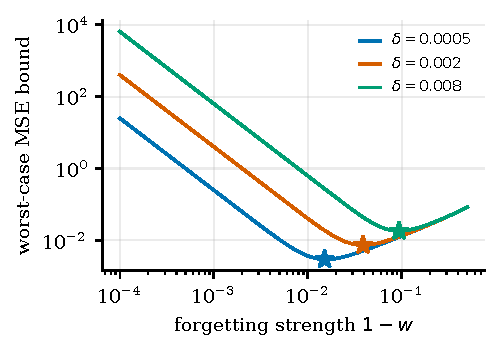
\includegraphics[width=0.93\linewidth]{figs/drift_tradeoff.pdf}
\caption{Bias--variance bounds in Proposition~\ref{prop:drift}. Stars
mark the minimizing forgetting strength; as drift $\delta$ increases,
the optimum moves at the rate in Corollary~\ref{cor:rate}.}
\label{fig:tradeoff}
\end{figure}

\subsection{Finite candidate selection}

\begin{proposition}[Conditional finite-class bound]
\label{prop:oracle}
Let $R(c)$ be the expected validation risk of candidate $c$ and
$\hat R(c)$ its average over $n$ validation items. If the item losses are
independent conditional on the fitted candidates and lie in $[0,B]$, then
the minimizer $\hat c$ over $M$ candidates satisfies, with probability at
least $1-\eta$,
\[
R(\hat c)\le\min_cR(c)+B\sqrt{\frac{2\log(2M/\eta)}{n}}.
\]
\end{proposition}

The independent units are items, because observations and quantiles are
averaged within item before selection. The released selector does not
clip scaled pinball loss, so the bounded-loss assumption is not automatic
and this proposition is not presented as a formal guarantee for the
unclipped implementation. It records the standard finite-class behavior
under an explicit clipping condition.

\subsection{Classical credibility}

\begin{proposition}[Pooling reduces Bayes risk in the stationary model]
\label{prop:credibility}
Under the undiscounted Beta--Binomial occurrence model with known
hyperparameters, the posterior mean is the Bayes estimator of $\pi_i$
under squared loss and has strictly smaller Bayes risk than the per-item
empirical rate whenever $\phi_g>0$. Its optimal weight is the classical
credibility factor $\lambda_i=n_i/(n_i+\phi_g)$
\citep{buhlmann1967}.
\end{proposition}

This is the B\"uhlmann--Straub result specialized to Bernoulli
occurrences. It justifies pooling when the stationary hierarchical model
is correctly specified; it does not assert that a misspecified or stale
group prior helps under drift.

\section{Proofs}\label{app:proofs}

\subsection{Proof of Proposition~\ref{prop:tsb-limit}}
(i) Immediate from \eqref{eq:disc-post} since $c(w),n(w)$ are finite.
(ii) Induction: $\hat p_1=(1-w)p_1+w\hat p_0$. If the closed form holds at
$T-1$, then
$\hat p_T=(1-w)p_T+w\hat p_{T-1}=(1-w)\sum_{t=1}^{T}w^{T-t}p_t+w^{T}\hat p_0$.
With $n(w)=(1-w^{T})/(1-w)$,
\[
\bar p(w)=\frac{(1-w)\sum_t w^{T-t}p_t}{1-w^{T}}
=\frac{\hat p_T-w^{T}\hat p_0}{1-w^{T}}.
\]
(iii) Rearranging, $\bar p(w)-\hat p_T=w^{T}(\bar p(w)-\hat p_0)$, and
$|\bar p(w)-\hat p_0|\le1$. \qed

\subsection{Proof of Proposition~\ref{prop:active}}
$n(w)=(1-w^{T})/(1-w)\le1/(1-w)$ and $x\mapsto x/(x+\phi)$ is increasing,
so $\lambda(w)\le[1/(1-w)]/[1/(1-w)+\phi]=1/(1+(1-w)\phi)$. \qed

\subsection{Proof of Proposition~\ref{prop:drift} and
Corollary~\ref{cor:rate}}
With $k=T-t$ and $\sum_{k\ge0}kw^k=w/(1-w)^2$,
\[
\bigl|\E\bar p(w)-\pi_T\bigr|
=\Bigl|\frac{\sum_t w^{T-t}(\pi_t-\pi_T)}{n(w)}\Bigr|
\le\frac{\delta\,w/(1-w)^2}{(1-w^{T})/(1-w)}
=\delta\,\frac{w}{(1-w)(1-w^{T})}.
\]
By independence and $\pi_t(1-\pi_t)\le\tfrac14$,
\[
\Var\,\bar p(w)\le\frac{\tfrac14\,(1-w^{2T})/(1-w^{2})}
{[(1-w^{T})/(1-w)]^{2}}
=\frac14\cdot\frac{(1-w)(1+w^{T})}{(1+w)(1-w^{T})}.
\]
Decomposing
$\hat\pi-\pi_T=\lambda(\bar p-\E\bar p)+\lambda(\E\bar p-\pi_T)+(1-\lambda)(\mu_\pi-\pi_T)$,
the first term is zero-mean and independent of the deterministic
remainder, giving
$\E(\hat\pi-\pi_T)^2\le[\lambda\mathrm{B}(w)+(1-\lambda)|\mu_\pi-\pi_T|]^2
+\lambda^2\Var\bar p(w)$ with $\mathrm{B}(w)$ the bias bound. For the
corollary set $b=1-w$ and let $T\to\infty$ (so $w^{T}\to0$): the squared
bias bound behaves as $\delta^2(1-b)^2/b^2\sim\delta^2/b^2$ and the
variance bound becomes $\tfrac14\, b/(2-b)$, which is $b/8$ to leading
order as $b\to0$. Minimizing $f(b)=\delta^2/b^2+b/8$ gives
$f'(b)=-2\delta^2/b^3+1/8=0$, i.e.,
$b^{*}=(16\delta^{2})^{1/3}=2^{4/3}\delta^{2/3}$, and
$f(b^{*})=O(\delta^{2/3})$. \qed

\subsection{Proof of Proposition~\ref{prop:oracle}}
For each candidate $c$, Hoeffding's inequality for independent scores in
$[0,B]$ gives
$\Pr\bigl(|\hat R(c)-R(c)|>t\bigr)\le2\exp(-2nt^2/B^2)$. A union bound
over the $M$ candidates makes
$\sup_c|\hat R(c)-R(c)|\le t$ hold with probability at least
$1-2M\exp(-2nt^2/B^2)$. Setting the right side to $\eta$ yields
$t=B\sqrt{\log(2M/\eta)/(2n)}$. On this event,
$R(\hat c)\le\hat R(\hat c)+t\le\hat R(c^{*})+t\le R(c^{*})+2t$ with
$c^{*}=\arg\min_c R(c)$, which is the claim with constant
$2t=B\sqrt{2\log(2M/\eta)/n}$. \qed

\subsection{Proof of Proposition~\ref{prop:credibility}}
With known $(\alpha_g,\beta_g)$ and $s_i\mid\pi_i\sim
\mathrm{Bin}(n_i,\pi_i)$, $\pi_i\sim\mathrm{Beta}(\alpha_g,\beta_g)$,
the posterior mean $\hat\pi_i=\lambda_i\bar p_i+(1-\lambda_i)\mu_\pi$
with $\lambda_i=n_i/(n_i+\phi_g)$ minimizes Bayes risk under squared
loss among all estimators (tower property). Restricting to linear
combinations $a\bar p_i+b$, the Bayes risk is
$a^2\,\E[\Var(\bar p_i\mid\pi_i)] + (1-a)^2\Var(\pi_i)$ at the optimal
intercept, minimized at
$a^{*}=\Var(\pi_i)/\bigl(\Var(\pi_i)+\E[\Var(\bar p_i\mid\pi_i)]\bigr)
=\lambda_i$, the B\"uhlmann credibility weight. The minimum is strictly
below the risk of $a=1$ (the empirical rate) whenever
$\Var(\pi_i)<\infty$ and $\phi_g>0$. \qed

\subsection{Proof of Proposition~\ref{prop:twosided} and
Corollary~\ref{cor:resolution}}

\textbf{(i)} $\lambda_i=n_i/(n_i+\kappa_g)$ is increasing in $n_i$, and
$n_i\le\sum_{k\ge0}w^{k}=(1-w)^{-1}$ for $w<1$. Substituting the bound,
$\lambda_i\le\frac{(1-w)^{-1}}{(1-w)^{-1}+\kappa_g}
=\bigl[1+(1-w)\kappa_g\bigr]^{-1}$, which is $<1$ whenever $w<1$ and
$\kappa_g>0$.

\textbf{(ii)} Write $\bar y_i=\mu_i+e_i$ with
$\mu_i\sim N(\mu_g,\tau_g^2)$ and $e_i\sim N(0,s_i)$ independent,
$s_i=\sigma_g^2/n_i$, so $\Var(\bar y_i)=\tau_g^2+s_i$. For the sample
variance $S_g^2=(m_g-1)^{-1}\sum_{i\in g}(\bar y_i-\bar{\bar y})^2$,
independence gives
$\Var(\bar{\bar y})=m_g^{-2}\sum_i(\tau_g^2+s_i)$ and hence
\[
\E[S_g^2]=\frac{\sum_i(\tau_g^2+s_i)-m_g\Var(\bar{\bar y})}{m_g-1}
=\frac{(1-m_g^{-1})\sum_i(\tau_g^2+s_i)}{m_g-1}
=\tau_g^2+\bar s_g ,
\]
exactly, with no balance assumption. The estimator truncates precisely
when $S_g^2\le\bar s_g$. Under the working model $S_g^2$ is
approximately $(\tau_g^2+\bar s_g)\chi^2_{m_g-1}/(m_g-1)$, so
$\Var(S_g^2)\simeq\frac{2}{m_g-1}(\tau_g^2+\bar s_g)^2$ and the
standardized distance from the truncation boundary is
\[
\frac{\E[S_g^2]-\bar s_g}{\sqrt{\Var(S_g^2)}}
=\frac{\tau_g^2}{\sqrt{2/(m_g-1)}\,(\tau_g^2+\bar s_g)}
=\sqrt{\tfrac{m_g-1}{2}}\;\rho_g ,
\]
giving the stated normal approximation for
$\Pr[S_g^2\le\bar s_g]$. The discount bound follows from
$n_i\le(1-w)^{-1}$: $s_i=\sigma_g^2/n_i\ge(1-w)\sigma_g^2$ for every
$i$, hence $\bar s_g\ge(1-w)\sigma_g^2$, and $\rho_g$ is decreasing in
$\bar s_g$. Finally $\hat\tau_g^2=0$ gives $\kappa_g=\infty$ and
$\lambda_i=0$.

\textbf{Corollary.} Requiring the collapse probability to stay below a
fixed level is, by (ii), the condition $\rho_g\sqrt{(m_g-1)/2}\ge c$ for
a constant $c$ of order one. Solving
$\rho_g=\tau_g^2/(\tau_g^2+\bar s_g)\ge c\sqrt{2/(m_g-1)}$ for
$\tau_g^2$ gives
$\tau_g^2\ge\bar s_g\,c\sqrt{2}/(\sqrt{m_g-1}-c\sqrt2)$, i.e.\ the
stated order $\bar s_g/(\sqrt{m_g-1}-1)$ up to the constant. Refining a
partition decreases $m_g$ and, by construction of the mixture objective,
$\tau_g^2$, while decreasing $w$ raises the floor $(1-w)\sigma_g^2$ on
$\bar s_g$. Each shrinks the left side or raises the right side. \qed

The algebraic steps, the exact unbiasedness in (ii), and the monotonicity
claims are verified with a computer algebra system in
the released test suite. The $\chi^2$ approximation in (ii) is checked
against Monte Carlo simulation, agreeing to within $0.05$ in probability
across the regimes we use.

\section{Implementation details}\label{app:implementation}

\paragraph{EB fitting.} Group Beta--Binomial hyperparameters maximize the
(weighted) marginal likelihood by L-BFGS-B with positivity bounds; the
size block uses pooled within-item variance for $\sigma^2_g$ and an
intercept-only restricted marginal likelihood in $\tau^2_g$ with profiled
$\mu_{0,g}$; item-level process variances use the conjugate
scaled-inv-$\chi^2$ update with $\nu{=}20$. With discounting, every count
is replaced by its weighted analogue \eqref{eq:discounted-stats}; the
Beta--Binomial marginal extends to real pseudo-counts via log-Gamma
functions. The predictive law is zero-inflated log-normal with predictive
variance $\hat\sigma^2_{\mathrm{proc}}+\hat v_\mu$. The released
configuration averages quantiles over $B{=}20$ bootstrap resamples of the
item-statistics rows. An optional location-scale calibration layer exists
but is \emph{off} in all headline results; the adaptive conformal
comparison is reported as a separate baseline rather than used to modify
\EBB{} after fitting.

\paragraph{Mixture EM.} Deterministic quantile initialization over
(occurrence rate, mean log-size); degenerate components (mass $<2$)
frozen to global fallback priors; tolerance $10^{-5}$, max 60 iterations;
$K\in\{1,\dots,6\}$ by BIC with $5K+(K-1)$ parameters.

\paragraph{Selection.} Internal chronological split (first 80\% / last
20\%, min head 8); score = mean pinball over $q\in\{0.5,0.75,0.9\}$,
per-series scaled by head mean absolute demand, averaged within item and then
uniformly across items; grid over
$w\in\{1,0.999,0.997,0.995,0.99,0.98,0.95,0.90\}$ and partitions
\{global, taxonomy, mixture(BIC)\}. Selected configurations per dataset
are reported beneath Table~\ref{tab:point}; diagnostics
(\texttt{remix\_selection\_diagnostics.csv}) accompany every run.

\paragraph{Environment and timing methodology.} All experiments ran on one
Windows~11 workstation (Intel Core Ultra~9 275HX, 32\,GB RAM). Core
determinism tests are bit-identical within this environment;
cross-environment bit identity is not claimed. Timing is wall-clock and
excludes data loading. Joint selection over the 24 candidates takes
$51$--$243$ seconds per panel, with one deterministic six-$K$ EM/BIC
search for the mixture on the fitting head. Final model-only point plus
five-quantile prediction with $B=20$ takes 6.2 seconds on
Carparts, 38.0 on Online Retail, and 124.0 on M5, whose
external span has 3.235 million observations. GPU is not used in \EBB{}.

\paragraph{Baselines.} StatsForecast defaults; TSB
$(\alpha_d,\alpha_p)=(0.5,0.45)$; AutoARIMA/AutoTheta season 7 (daily) /
12 (monthly) for intervals. TSB-tuned: $5\times5$ grid
$\alpha_d\in\{0.05,0.1,0.2,0.35,0.5\}$,
$\alpha_p\in\{0.01,0.05,0.1,0.25,0.45\}$ (25 candidates, the same order
as \EBB{}'s 24), scored on the identical 80/20 chronological split by
per-series scaled MAE (so neither method is scored on its home
criterion), refit on the full window. Selected $(\alpha_d,\alpha_p)$:
Online Retail $(0.10,0.25)$; M5 $(0.20,0.01)$; Auto $(0.20,0.10)$;
Carparts $(0.50,0.45)$, i.e.\ the textbook constants; RAF
$(0.50,0.25)$. Static conformal wrappers use a chronological 80/20 split
and a \emph{panel-pooled} signed-residual distribution; quantiles are
zero-truncated and monotonized. The ACI variants retain that residual
pool and adapt the requested level for every series--quantile pair with
$\gamma=0.05$. Tweedie-GLM is a per-series autoregressive GLM with log
link, $p{=}1.5$, 14 lags (daily) / 6 (monthly), and $\ell_2{=}0.1$.
TweedieGP uses the authors' official implementation with Tweedie
likelihood, median-demand scaling, RBF kernel, and 50{,}000 predictive
samples; zero-only training series receive a zero fallback so that every
series is scored. iETS uses \texttt{smooth::adam} with automatic
occurrence modeling.


\section{Main-text material in full}\label{app:demoted}

This appendix keeps, verbatim, the tables, figures, and paragraphs of the
long-form manuscript that the main text summarizes.

\subsection{The two coupled choices in real data}
\begin{figure*}[t]
\centering
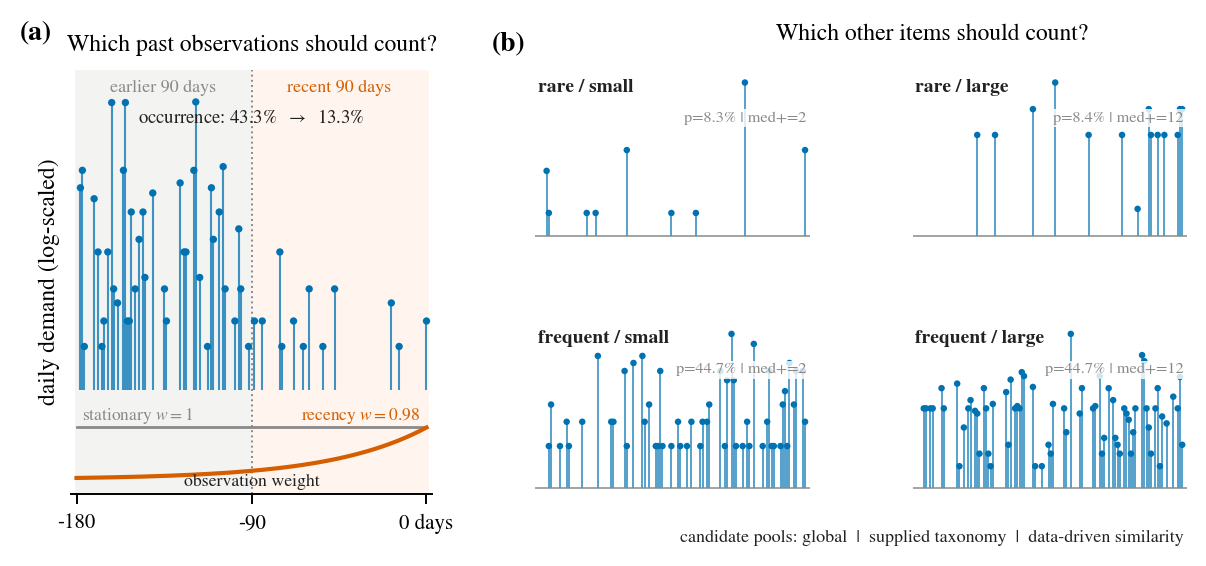
\includegraphics[width=0.98\textwidth]{fig01_problem.png}
\caption{The two coupled choices, in real intermittent demand.
\textbf{(a)} One item's daily history: occurrence falls from $43.3\%$ to
$13.3\%$ between the earlier and the recent ninety days, so a stationary
weighting ($w=1$) and a recency weighting ($w=0.98$) summarize the same
history differently---which past observations should count?
\textbf{(b)} Four items from the same panel, spanning rare and frequent
occurrence at small and large sizes: any pooled prior must decide which
of these heterogeneous neighbors an item should borrow strength
from---which other items should count? Candidate pools are a global
pool, a supplied taxonomy, and data-driven similarity.}
\label{fig:problem}
\end{figure*}

\subsection{Persistent prior leverage}

Fix an item and suppress its subscripts. Because
$n(w)=\sum_{t=1}^{T}w^{T-t}\le(1-w)^{-1}$ for $w<1$, the occurrence
credibility weight cannot converge to one.

\begin{proposition}[Forgetting keeps pooling relevant]
\label{prop:active}
For every horizon $T$,
$\lambda(w)\le\{1+(1-w)\phi\}^{-1}<1$ when $w<1$, whereas
$\lambda(1)\to1$ as $T\to\infty$. Hence the pooled occurrence prior
retains positive weight indefinitely under forgetting.
\end{proposition}

The statement is about leverage, not benefit: it does not guarantee
that a particular prior is a good shrinkage target. It says that the
choice of target can continue to affect forecasts even for old series.


\subsection{Resolution diagnostics recorded by the selector}
Fitting each candidate already produces everything the resolution
analysis of Section~\ref{sec:resolution} needs, so the selector records it
rather than recomputing it later. For every $(r,w)$ and every resulting
group $g$ we store, from the fitting head only, the median occurrence and
positive-size credibility weights $\lambda_i^{(o)}$ and $\lambda_i^{(+)}$,
the share of items with $\lambda_i^{(+)}<0.1$, the group sizes $m_g$, and
the resolution statistic
\[
\hat z_g=\frac{S_g^2-\bar s_g}{\sqrt{2/(m_g-1)}\,S_g^2},
\]
whose nonpositive values coincide with the collapse event
$\hat\tau_g^2=0$ of Proposition~\ref{prop:twosided}. These quantities cost
nothing beyond the fit that produced them, they are computed before any
external observation is seen, and they answer a question the validation
score cannot: not which candidate scores best on the tail, but whether the
discounted data contain enough information to estimate the candidate's
group structure at all. Section~\ref{sec:main-results} uses them to
separate the two. The full selection surface and the accompanying
diagnostics are released with every run
(\texttt{remix\_selection\_diagnostics.csv}).


\subsection{Pooling candidates and computational profile}
Let $\mathcal R$ contain three ways to construct $g(\cdot)$ from the
fitting data. Table~\ref{tab:pool-candidates} orders them from coarse to
fine: one prior for the panel, one prior per fixed demand-pattern class,
and one prior per learned component. The ladder is deliberate. The
question this paper asks is not which rung is best in general---that
depends on the panel---but whether the discounted data support moving up
it at all. Section~\ref{sec:resolution} gives the condition under which
they do, and Section~\ref{sec:main-results} reports what happens when they
do not.

\begin{table}[t]
\centering
\caption{Pooling candidates used by \EBB{}, ordered coarse to fine.
Every data-dependent label is computed from the selector's fitting head,
never its validation tail.}
\label{tab:pool-candidates}
\small
\setlength{\tabcolsep}{3.5pt}
\begin{tabular}{lp{0.70\linewidth}}
\toprule
Candidate & Shared-prior groups\\
\midrule
Global & All items share one prior.\\
Taxonomy & Four ADI/CV$^2$ demand-pattern classes (smooth, intermittent,
erratic, lumpy) using the classical thresholds $1.32$ and $0.49$
\citep{syntetos2005categorization}.\\
Learned & Hard assignments from a mixture of occurrence--size prior
components; $K\in\{1,\ldots,6\}$ is selected by BIC.\\
\bottomrule
\end{tabular}
\end{table}

For the learned candidate, component $k$ carries
$\eta_k=(\alpha_k,\beta_k,\mu_{0,k},\tau_k^2,\sigma_k^2)$. Its item
marginal is the product of Beta--Binomial occurrence evidence and Normal
random-effects size evidence. EM has an analytic responsibility update;
its M-step maximizes responsibility-weighted EB objectives. A
deterministic quantile initialization makes repeated fits seed-free.
Mixture labels are built once from the fitting head and shared across the
discount grid, with $K\in\{1,\dots,6\}$ selected by BIC at that fit.
Re-learning the partition separately at every discount is a natural
variant---changing $w$ changes both the item evidence and the components
it can support---but we do not evaluate it here. The
selected responsibilities are converted to hard labels so all three
candidates share the same downstream forecaster.



Two properties of this cost profile matter for the comparisons that
follow. First, the whole pipeline is CPU-only and closed form apart from
the mixture search: fitting and predicting a panel costs on the order of
milliseconds per series, so the full 24-candidate joint selection
completes in minutes on a laptop-class machine and no GPU, tuning budget,
or convergence diagnostic is required. Second, estimation is exact rather
than approximate at every stage, so repeated end-to-end runs are
bit-identical in the released test suite. Neither property is an accuracy
claim; both are the terms on which the accuracy results in
Section~\ref{sec:experiments} should be read, since several of the
strongest comparators there cost two to three orders of magnitude more per
series and none is reproducible to the bit. Measured wall-clock figures
for every method are in Appendix~\ref{app:implementation}.

\subsection{Fixed-origin results in full}
\label{sec:main-results}
% =========================================================================

\begin{table*}[t]
\centering
\caption{\textbf{Probabilistic forecasting is the primary comparison.}
Scaled pinball loss (SPL; lower is better) is reported as the mean over
$q\in\{0.1,0.25,0.5,0.75,0.9\}$ and at q90. Bold and underline mark the
best and second-best non-degenerate methods. M5 reports seed 42 for direct
comparability; three-seed robustness is summarized in the text. \EBB{}
uses its raw predictive law, with no post-hoc calibration. TweedieGP is the
official implementation of Damato et al.\ at its released defaults on
all five panels; Appendix~\ref{app:efficiency} reports measured cost.
The all-zero row is a metric diagnostic and
is excluded from ranking.}
\label{tab:prob}
\small
\setlength{\tabcolsep}{3.2pt}
\begin{tabular}{lcc@{\hspace{9pt}}cc@{\hspace{9pt}}cc@{\hspace{9pt}}cc@{\hspace{9pt}}cc}
\toprule
 & \multicolumn{2}{c}{Online Retail} & \multicolumn{2}{c}{M5} & \multicolumn{2}{c}{Auto} & \multicolumn{2}{c}{Carparts} & \multicolumn{2}{c}{RAF}\\
\cmidrule(lr){2-3}\cmidrule(lr){4-5}\cmidrule(lr){6-7}\cmidrule(lr){8-9}\cmidrule(lr){10-11}
Model & Mean & q90 & Mean & q90 & Mean & q90 & Mean & q90 & Mean & q90\\
\midrule
AutoARIMA & 1.0069 & 1.6297 & 1.7919 & 2.4148 & 0.3189 & 0.2659 & 0.4084 & 0.4897 & 0.4020 & 0.5910\\
AutoTheta & 1.0055 & 1.6056 & 1.7954 & 2.3123 & 0.3403 & 0.2760 & 0.3925 & \secondbest{0.4697} & 0.4104 & 0.5956\\
CP-Croston & 1.5502 & 2.7686 & 1.6902 & \best{2.1551} & 0.3260 & 0.3105 & 0.4012 & 0.5433 & 0.3322 & 0.4927\\
CP-SBA & 1.5492 & 2.8601 & 1.6939 & 2.1736 & 0.3256 & 0.3153 & 0.3982 & 0.5418 & 0.3290 & 0.4920\\
CP-TSB & 1.1744 & 2.6746 & 1.8794 & 2.3148 & 0.3459 & 0.3150 & 0.3783 & 0.4842 & 0.3814 & 0.4986\\
CP-ADIDA & 1.1239 & 2.5409 & 1.7150 & 2.1949 & 0.3275 & 0.3082 & 0.3571 & 0.4982 & 0.3097 & 0.4905\\
CP-IMAPA & 1.1280 & 2.5506 & 1.7190 & 2.1904 & 0.3279 & 0.3084 & 0.3561 & 0.4908 & 0.3116 & 0.4907\\
Tweedie-GLM & 1.1477 & 1.7458 & 4.0693 & 5.2620 & 0.3221 & 0.2783 & 0.4776 & 0.6897 & 0.3121 & 0.5312\\
iETS & 0.9846 & 1.7544 & 2.0282 & 2.9772 & 0.3448 & 0.3252 & 0.4561 & 0.5646 & 0.3494 & \secondbest{0.4900}\\
TweedieGP & \best{0.8845} & \best{1.5218} & \best{1.6228} & \secondbest{2.1723} & \secondbest{0.2985} & \best{0.2598} & \best{0.3214} & \best{0.4600} & \secondbest{0.2763} & 0.5219\\
\midrule
Zero (diagnostic) & 0.9161 & 1.6490 & 1.9590 & 3.5262 & 0.5612 & 1.0102 & 0.3736 & 0.6725 & 0.2669 & 0.4805\\
\midrule
\EBB{} (ours) & \secondbest{0.8849} & \secondbest{1.5268} & \secondbest{1.6707} & 2.4758 & \best{0.2937} & \secondbest{0.2599} & \secondbest{0.3229} & 0.4817 & \best{0.2680} & \best{0.4856}\\
\bottomrule
\end{tabular}
\end{table*}

Table~\ref{tab:prob} sets the empirical position, and it is a narrow one.
\EBB{} attains the lowest mean SPL on Auto and RAF, by $1.6\%$ and
$3.0\%$ over the official TweedieGP implementation, both significant
(Table~\ref{tab:spl-significance}); TweedieGP attains it on Online Retail,
Carparts, and M5, by $0.05\%$, $0.5\%$, and $2.9\%$, of which only the M5
margin is significant. Against every other comparator \EBB{} is best on
all five panels, by $10.1\%$ over iETS on Online Retail and $1.2\%$ over
CP-Croston on M5. Across three independent
5{,}000-series M5 samples the selected configuration is identical---%
$(\text{mixture},\,w{=}0.95,\,K{=}6)$---and \EBB{} has mean SPL
$1.7501\pm0.084$ against $1.7547\pm0.065$ for CP-Croston, its closest
comparator: ahead on two samples, behind by $1.0\%$ on the third, and
ahead on average by $0.3\%$, well within one standard deviation. We report
the spread rather than an aggregate win because it is the quantity
Section~\ref{sec:leverage} explains. The explanation is not that these
panels leave no room for a hierarchical construction to work; on three of
them the credibility weights say otherwise. It is that the room which
exists is not converted by a learned partition, which is why the
achievable margin is set by the shared predictive law rather than by the
pooling structure.

The degenerate row exposes what the central quantiles cannot see. On RAF,
the all-zero forecast is marginally better through q90 because the true
quantiles of most series are zero. At $q\in\{0.95,0.975,0.99\}$ it falls
behind every intensity-bearing method, and intensity-bearing models become
distinguishable from one another (Appendix~\ref{app:fartail}). TweedieGP
is strongest throughout the Carparts far tail and remains competitive on
RAF. The probabilistic claim is therefore not that one distribution wins
every quantile, but that \EBB{} is the most consistent aggregate
performer across panels and remains informative in the region where a zero
forecast ceases to be useful.

Point forecasts tell a deliberately weaker story. \EBB{} is best on six
of ten MAE/RMSSE cells and top two on seven, but the zero forecast has the
lowest MAE on three panels and classical methods lead several remaining
cells. We report the complete point table and horizon decomposition in
Appendix~\ref{app:point}: they establish competitiveness and rule out a
long-horizon averaging artifact, but do not support uniform point-forecast
superiority.

% =========================================================================


\subsection{Walk-forward results in full}
\label{sec:walkforward}
% =========================================================================

\begin{table*}[t]
\centering
\caption{\textbf{Strict probabilistic walk-forward evaluation on all five
panels.} Online Retail and M5 use seven-day blocks; Auto, Carparts, and
RAF use monthly blocks. Mean and q90 are scaled pinball losses; all five
quantiles, coverage, and interval width are reported in
Appendix~\ref{app:walkforward}. Classical wrappers and ACI refit each
block. AutoARIMA, AutoTheta, iETS, and TweedieGP refit every four blocks
on Online Retail and every block on the monthly panels; on M5 these four
were not run under this protocol on cost grounds (dashes). \EBB{} updates
sufficient statistics each block; ACI-\EBB{} applies the ACI-ADIDA
calibration layer to \EBB{}'s predictive quantiles, and \EBB{} (rule)
applies it only where the validation-tail rule selects it, so it equals
one of the two rows above it on each panel and is not ranked. Bold and underline
rank non-degenerate methods by SPL; on RAF the all-zero forecast is
marginally lower than every method through q90. On M5, the longest daily
panel, the adaptive conformal layer decides the ranking: ACI-\EBB{} leads,
ACI-ADIDA is second, and uncalibrated \EBB{} is third.}
\label{tab:wfprob}
\footnotesize
\setlength{\tabcolsep}{3.0pt}
\begin{tabular}{lrrrrrrrrrr}
\toprule
 & \multicolumn{2}{c}{Online Retail} & \multicolumn{2}{c}{Carparts} & \multicolumn{2}{c}{Auto} & \multicolumn{2}{c}{RAF} & \multicolumn{2}{c}{M5}\\
\cmidrule(lr){2-3}\cmidrule(lr){4-5}\cmidrule(lr){6-7}\cmidrule(lr){8-9}\cmidrule(lr){10-11}
Model & Mean & q90 & Mean & q90 & Mean & q90 & Mean & q90 & Mean & q90\\
\midrule
AutoARIMA & 1.0627 & 1.5225 & 0.4195 & 0.4839 & 0.3139 & 0.2632 & 0.4083 & 0.5920 & --- & ---\\
AutoTheta & 1.0586 & 1.4835 & 0.4056 & 0.4743 & 0.3224 & 0.2619 & 0.4308 & 0.6233 & --- & ---\\
iETS & 1.1092 & 1.9404 & 0.4362 & 0.5154 & 0.3286 & 0.3009 & 0.3537 & 0.4902 & --- & ---\\
CP-TSB & 1.3733 & 2.8422 & 0.3836 & 0.4758 & 0.3297 & 0.3009 & 0.3842 & 0.4941 & 1.6616 & 2.0422\\
CP-ADIDA & 1.1576 & 2.5143 & 0.3509 & 0.4880 & 0.3175 & 0.2949 & 0.3095 & \secondbest{0.4894} & 1.5537 & 1.9629\\
CP-IMAPA & 1.1773 & 2.5224 & 0.3492 & 0.4789 & 0.3176 & 0.2948 & 0.3127 & 0.4903 & 1.5457 & 1.9490\\
ACI-ADIDA & 0.9108 & 1.6681 & 0.3417 & 0.4767 & 0.3147 & 0.2900 & 0.3085 & 0.5598 & \secondbest{1.4192} & \secondbest{1.8064}\\
TweedieGP & \best{0.8526} & \best{1.3791} & \best{0.3121} & \best{0.4326} & 0.2924 & \best{0.2539} & 0.2801 & 0.5261 & --- & ---\\
Zero (diagnostic) & 0.9161 & 1.6490 & 0.3736 & 0.6725 & 0.5612 & 1.0102 & 0.2669 & 0.4805 & 1.9590 & 3.5262\\
\midrule
\EBB{} & \secondbest{0.8540} & \secondbest{1.4002} & 0.3145 & 0.4578 & \secondbest{0.2910} & 0.2563 & \best{0.2681} & \best{0.4864} & 1.4851 & 1.8797\\
ACI-\EBB{} & 0.9082 & 1.5623 & \secondbest{0.3128} & \secondbest{0.4521} & \best{0.2901} & \secondbest{0.2560} & \secondbest{0.2743} & 0.5175 & \best{1.3785} & \best{1.6438}\\
\EBB{} (rule) & 0.8540 & 1.4002 & 0.3145 & 0.4578 & 0.2901 & 0.2560 & 0.2681 & 0.4864 & 1.3785 & 1.6438\\
\bottomrule
\end{tabular}
\end{table*}

Table~\ref{tab:wfprob} is the deployment-facing test, and it reproduces
the fixed-origin picture for the uncalibrated methods. \EBB{} leads on
Auto and RAF, by $0.5\%$ and $4.3\%$ over TweedieGP; TweedieGP leads on
Online Retail and Carparts by $0.2\%$ and $0.8\%$. Per-series paired tests
(Table~\ref{tab:wf-significance}) cannot separate the two on Online
Retail, Carparts, or Auto, and favor \EBB{} on RAF. Over adaptive
conformal inference on ADIDA, \EBB{} gains $6.2\%$ on Online Retail and
$8.0\%$ on Carparts, beats every static conformal wrapper on all five
panels, and loses M5 by $4.4\%$.

The M5 loss is a calibration effect, and the same layer is available to
\EBB{}. ACI-\EBB{} reads \EBB{}'s predictive quantile at the adaptive
level instead of the nominal one. On M5 it lowers mean SPL from $1.4851$
to $1.3785$, $2.9\%$ below ACI-ADIDA and significant; it also leads Auto
($0.2901$) and brings Carparts to within $0.2\%$ of TweedieGP. On Online
Retail and RAF the same layer hurts, by $6.3\%$ and $2.3\%$, because the
per-series coverage signal is too noisy on those panels to improve an
already calibrated forecaster. Whether to apply it is therefore a
selection problem, and the initialization window already answers it: on
the same 80/20 chronological split used to select the discount, \EBB{} is
walked forward over the validation tail with and without the layer, and
the layer is applied iff its tail pinball is lower
(Appendix~\ref{tab:aci-rule}). The rule applies the layer on M5 and Auto
and withholds it elsewhere, matching the ex-post better variant on
4 of five panels (Carparts is the exception, where the two
are within $0.5\%$ and statistically undecided), and the tail gains it
sees track the external ones ($+7.8\%$ versus $+7.2\%$ on M5, $-7.9\%$
versus $-6.3\%$ on Online Retail). The resulting row, \EBB{} (rule), is
within 0.8\% ({Carparts}) of the best competing method on every
panel under walk-forward updating. Two further facts survive the mixed
result: under equal calibration \EBB{} beats the ADIDA base on all five
panels (undecided only on Online Retail), and the adaptive layer's benefit
is a property of the panel, not of the forecaster it wraps.

Table~\ref{tab:regret} and Figure~\ref{fig:frontier} summarize both
protocols by the largest shortfall to the per-panel best. Against
competing methods, \EBB{} and TweedieGP are the only ones within five
percent everywhere (\EBB{} at most $3.0\%$ at fixed origin and $4.6\%$
under walk-forward updating; TweedieGP $3.1\%$ and $4.5\%$), and every
other method is at least $15\%$ behind on some panel. Counting our own
wrapper as a competitor, uncalibrated \EBB{} trails ACI-\EBB{} by $7.7\%$
on M5, and \EBB{} (rule) closes that to 0.8\%. The two leaders differ in cost. TweedieGP refits per-series
variational GPs at every update, so its walk-forward runs took between
$36$ minutes (Auto) and $2.4$ hours (RAF) with twelve workers and project
to about $51$ hours on M5 at the Online Retail cadence; \EBB{} updates
sufficient statistics in closed form and completes each of the five
walk-forward runs in under $40$ seconds on one core, and ACI-\EBB{} adds
a few seconds (Table~\ref{tab:wfcost}).

\begin{table}[t]
\centering
\caption{\textbf{Largest shortfall to the per-panel best.} For each
method, the maximum over panels of its mean-SPL regret to the best
non-degenerate method on that panel (percent; the panel attaining it in
parentheses; Carp.\ is Carparts), and the number of panels on which the method is within
$5\%$ of the best. A superscript gives the number of panels evaluated
when fewer than five. ACI-\EBB{} and the rule row exist only under walk-forward updating; the
rule row is excluded from the per-panel best.
Per-panel regrets are in Table~\ref{tab:regret-full}.}
\label{tab:regret}
\footnotesize
\setlength{\tabcolsep}{2.6pt}
\begin{tabular}{lcccc}
\toprule
 & \multicolumn{2}{c}{Fixed origin} & \multicolumn{2}{c}{Walk-forward}\\
\cmidrule(lr){2-3}\cmidrule(lr){4-5}
Method & Max (panel) & $\le5\%$ & Max (panel) & $\le5\%$\\
\midrule
AutoARIMA & 50.0 (RAF) & 0/5 & 52.3 (RAF)$^{4}$ & 0/4\\
AutoTheta & 53.1 (RAF) & 0/5 & 60.7 (RAF)$^{4}$ & 0/4\\
Tweedie-GLM & 150.8 (M5) & 0/5 & --- & ---\\
iETS & 41.9 (Carp.) & 0/5 & 39.8 (Carp.)$^{4}$ & 0/4\\
CP-Croston & 75.3 (OR) & 1/5 & 60.9 (OR) & 0/5\\
CP-SBA & 75.1 (OR) & 1/5 & 61.5 (OR) & 0/5\\
CP-TSB & 42.3 (RAF) & 0/5 & 61.1 (OR) & 0/5\\
CP-ADIDA & 27.1 (OR) & 0/5 & 35.8 (OR) & 0/5\\
CP-IMAPA & 27.5 (OR) & 0/5 & 38.1 (OR) & 0/5\\
ACI-ADIDA & --- & --- & 15.1 (RAF) & 1/5\\
TweedieGP & 3.1 (RAF) & 5/5 & 4.5 (RAF)$^{4}$ & 4/4\\
\midrule
\EBB{} & 3.0 (M5) & 5/5 & 7.7 (M5) & 4/5\\
ACI-\EBB{} & --- & --- & 6.5 (OR) & 4/5\\
\EBB{} (rule) & --- & --- & 0.8 (Carp.) & 5/5\\
\bottomrule
\end{tabular}
\end{table}

\begin{figure*}[t]
\centering
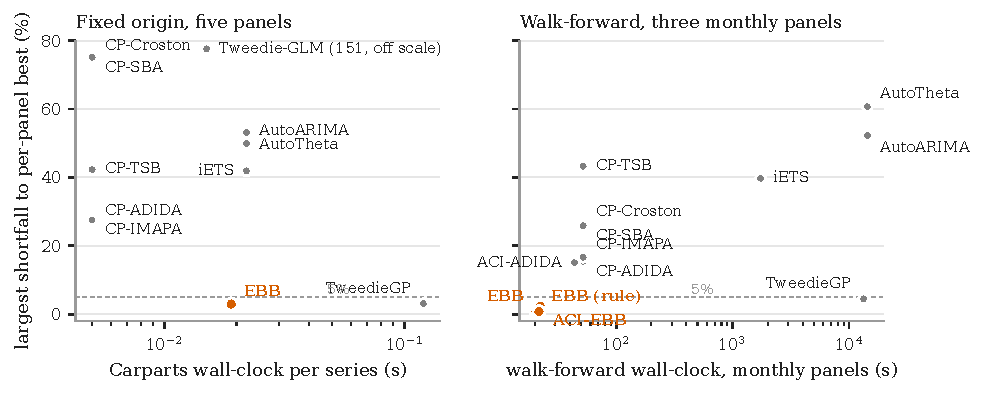
\includegraphics[width=0.96\textwidth]{figs/fig12_frontier.pdf}
\caption{\textbf{Largest shortfall against cost.} Each point is one
method; $y$ is its largest mean-SPL shortfall to the per-panel best
(Table~\ref{tab:regret}), $x$ is measured wall-clock on a log scale.
Left: fixed origin over five panels against Carparts cost per series
(Table~\ref{tab:efficiency}). Right: walk-forward over the three monthly
panels, on which every method has a measured wall-clock, against the total
walk-forward wall-clock on those panels (Table~\ref{tab:wfcost}; TweedieGP
uses twelve workers, every other method one process). The dashed line
marks $5\%$.}
\label{fig:frontier-full}
\end{figure*}



The configuration is selected once at the origin and then updated online;
repeated online re-selection is outside the present experiment.

% =========================================================================


\subsection{Controlled test of the resolution mechanism}

\label{sec:synthetic}
% =========================================================================

Real data never reveal the true pooling partition, so on their own they
cannot distinguish a partition that is not worth having from one we failed
to find. Both appear as a small number. We therefore construct panels
where the partition is correct by definition, and use them as a reference
against which the learned partitions of Section~\ref{sec:leverage} are
measured: what a good partition is worth at a given level of credibility
leverage, rather than what our estimator obtains there.

We simulate from the hierarchical hurdle model of \eqref{eq:model} with
group centers arranged symmetrically around a fixed grand mean, so that
increasing separation does not change the panel scale. Each cell compares
a single pool against the known true partition under the same predictive
representation, with nine paired replicates, and sweeps the two quantities
that Section~\ref{sec:resolution} identifies as controlling credibility:
the discount $w$ and the series length $T$. The resulting grid spans the
leverage range the real panels occupy, from the near-fully-shrunk regime
of Carparts to the item-dominated regime of Auto and RAF.

\begin{table*}[t]
\centering
\caption{Advantage of the \emph{true} partition over a single pool on
simulated panels (mean percentage improvement over nine paired replicates;
standard error in parentheses). Positive favors the partition. $T$ is
series length.}
\label{tab:sanity}
\small
\setlength{\tabcolsep}{3.5pt}
\begin{tabular}{llrrrr}
\toprule
$T$ & $w$ & NLL & log-size MSE & pinball & MAE\\
\midrule
$30$ & $0.90$ & $2.40\;(0.18)$ & $17.15\;(2.39)$ & $2.25\;(0.61)$ & $-1.72\;(0.73)$\\
$30$ & $0.95$ & $1.12\;(0.39)$ & $9.00\;(2.45)$ & $-0.44\;(0.58)$ & $-0.17\;(0.51)$\\
$30$ & $1.00$ & $1.02\;(0.08)$ & $8.37\;(1.53)$ & $-0.69\;(0.32)$ & $-1.95\;(0.59)$\\
$120$ & $0.90$ & $1.65\;(0.22)$ & $18.36\;(1.56)$ & $1.57\;(0.64)$ & $-3.34\;(1.37)$\\
$120$ & $0.95$ & $0.96\;(0.11)$ & $3.65\;(0.77)$ & $0.23\;(0.28)$ & $-1.32\;(0.73)$\\
$120$ & $1.00$ & $0.23\;(0.04)$ & $1.13\;(0.31)$ & $-0.32\;(0.13)$ & $-0.80\;(0.11)$\\
\bottomrule
\end{tabular}
\end{table*}

Table~\ref{tab:sanity} gives the result. The true partition improves NLL
and log-size MSE in every cell, and pinball loss whenever forgetting is
strong; in a separate length sweep its pinball advantage decays from
$1.53\%$ at $T=12$ to $0.01\%$ at $T=400$. Both patterns follow the
credibility mechanism directly. Discounting or short histories reduce an
item's own weight $\lambda^{(+)}_i$ and open room for a prior to act;
long undiscounted histories drive $\lambda^{(+)}_i\to1$ and make every
partition irrelevant. Stronger forgetting simultaneously makes group
variance components harder to estimate, as
Proposition~\ref{prop:twosided} predicts, which is why the gains in the
$w=0.90$ rows are bought against a noisier $\hat\tau_g^2$ and do not
continue to grow without limit. Extending the grid with a separation axis
(Appendix~\ref{app:simulation-details}; group centers $0$ to $3$
log-units apart) shows that the return is governed by the forgetting
regime as much as by leverage: with no separation in either block the return is within noise of
zero; with $w=0.90$ a true partition earns $1$--$2.7\%$ from separation
$0.5$ upward, with $w=0.95$ it exceeds $1\%$ only at separation $0.5$
with long histories ($\lambda^{(+)}\approx0.4$), and with $w=1$ it never
does. The learned mixture, run on the same simulated panels, is negative
at every moderate separation, and the two remedies already in the code
base---label sample-splitting and credibility shrinkage of the group
variance---do not recover the loss (grid means $-0.58\%$, $-0.79\%$, $-0.66\%$, and $-0.56\%$ combined).

MAE moves the other way in all six cells. A known-correct partition, on
data generated from the model it describes, is reported as harmful by the
metric most commonly used in this literature. We take this as the cleanest
available statement of why Section~\ref{sec:main-results} treats
absolute-error criteria as diagnostics rather than as the headline.

\paragraph{What these panels are for.}
Plotted against median $\lambda^{(+)}$, the cells of
Table~\ref{tab:sanity} and the length sweep trace the grey curves of
Figure~\ref{fig:refinement-leverage}: the return to \emph{correct}
structure as a function of leverage. Because the partition is supplied
rather than estimated, that return is an upper envelope---no procedure
that must also learn the grouping can exceed it, and any procedure that
falls below it is losing something to estimation rather than to a lack of
structure. This is the comparison Section~\ref{sec:leverage} draws, and it
is the reason the controlled study is necessary rather than decorative:
the real panels supply the leverage coordinates, and only a known-partition
experiment can supply the ordinate they should be judged against.

Two boundaries apply. The experiment isolates the value of correct
structure and says nothing about whether the mixture recovers it---indeed
Section~\ref{sec:leverage} shows it does not, and the gap between the two
is precisely what the comparison measures. And it simulates from the model
that \EBB{} fits, so the mechanism is tested under correct specification
only; a misspecified size law would shift the envelope, though it is hard
to see how it would raise it. Full diagnostics, including the growth of
$\mathrm{RMSE}(\hat\tau_g^2)$ as $w$ falls, are in
Appendix~\ref{app:simulation-details}.

% =========================================================================


\subsection{Leverage, selection, and ablation}
\label{sec:leverage}
% =========================================================================

The results so far are consistent and small. This section asks whether
their size is a property of the data or of our estimator, and shows that
the two can be told apart with quantities the selector already computes on
the fitting head (Section~\ref{sec:select}).

\paragraph{What gets selected, and how weakly.}
All five panels select $w<1$: Carparts $0.90$, Online Retail and M5
$0.95$, Auto $0.99$, and RAF $0.997$. Across three independent
5{,}000-series M5 samples the selected configuration is identical in
structure, discount, and mixture order---$(\text{mixture},\,w{=}0.95,\,
K{=}6)$ in every case.

The pooling axis behaves differently, and the honest summary is that it
barely resolves. On three panels the spread between the best and worst
pooling structure at the selected discount is under a tenth of a percent
of validation SPL: $0.05\%$ on Online Retail, $0.08\%$ on Carparts,
$0.02\%$ on RAF. Only two panels separate at all---M5, where the learned
mixture beats the global pool by $0.58\%$, and Auto, where the global pool
beats every refinement by $0.31\%$. Announcing a winner on the other three
would report selector noise. What the selector reliably does is choose a
discount and avoid poor structural corners; it does not discover demand
taxonomies, and we do not claim it does.

\begin{table*}[t]
\centering
\caption{\textbf{Credibility leverage under a single pool.} Median
credibility weight per panel at no forgetting and at the selected
discount, for both blocks of the hurdle model:
$\lambda^{(o)}_i=n_i/(n_i+\phi_g)$ for occurrence and
$\lambda^{(+)}_i=n_i^{+}/(n_i^{+}+\kappa_g)$ for positive size, the
latter being the quantity bounded by Proposition~\ref{prop:twosided}.
A weight near one means the item's own history dominates its posterior,
bounding how far any shared prior can move it. ``$<0.1$'' is the share of
items whose size-block weight falls below $0.1$. The final column is the
external MAE change of a separately selected learned partition relative to
the single pool; negative favors the single pool.}
\label{tab:leverage}
\small
\setlength{\tabcolsep}{3.0pt}
\begin{tabular}{lccccccc}
\toprule
 & & \multicolumn{3}{c}{$\lambda^{(+)}$ (size)} & \multicolumn{2}{c}{$\lambda^{(o)}$ (occ.)} & learned\\
\cmidrule(lr){3-5}\cmidrule(lr){6-7}
Panel & $w^{*}$ & $w{=}1$ & $w^{*}$ & $<0.1$ & $w{=}1$ & $w^{*}$ & vs.\ pool\\
\midrule
Carparts & $0.90$ & 0.802 & \textbf{0.224} & 22.5\% & 0.882 & 0.628 & $-1.2\%$\\
Online Retail & $0.95$ & 0.897 & \textbf{0.553} & 14.6\% & 0.969 & 0.895 & $-2.9\%$\\
M5 & $0.95$ & 0.996 & 0.841 & 12.9\% & 0.998 & 0.931 & $-2.3\%$\\
Auto & $0.99$ & 0.944 & 0.940 & 0.0\% & 0.525 & \textbf{0.422} & $-3.6\%$\\
RAF & $0.997$ & 0.926 & 0.917 & 0.0\% & 0.085 & \textbf{0.106} & $-31.5\%$\\
\bottomrule
\end{tabular}
\end{table*}

\paragraph{Leverage is an upper bound, not a prediction.}
Table~\ref{tab:leverage} reports the diagnostic. Read as
Corollary~\ref{cor:resolution} intends, it does not say which partition
wins; it says how much any partition could win by. Two panels have almost
no room on the size block: Auto and RAF retain median
$\lambda^{(+)}\approx0.92$--$0.94$ even at their selected discounts, with
no item below $0.1$, so their sub-percent pooling differences are
explained before any partition is fitted. % [ORIG 2026-09-13]
The remaining three retain
leverage: Carparts is extreme---median $0.224$, with $22.5\%$ of items
essentially fully shrunk---and Online Retail sits at $0.553$ under the
selected discount. Leverage alone does not fix the prize, however. The
controlled study shows that the true partition's return at a given
$\lambda^{(+)}$ depends on the forgetting regime that produced it and on
how far the groups are apart, so the panels are placed on the full
surface below.

\begin{figure}[t]
\centering
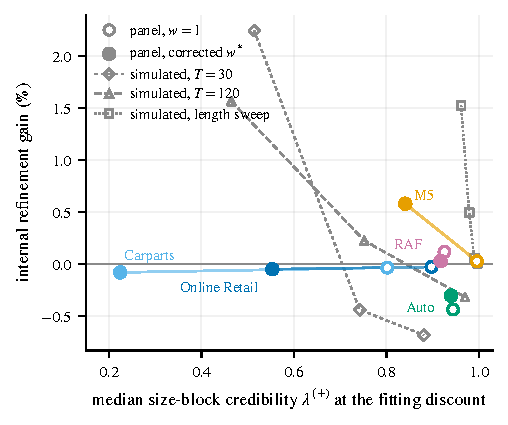
\includegraphics[width=\columnwidth]{figs/fig10a_refinement_leverage_size.pdf}\\[0.5em]
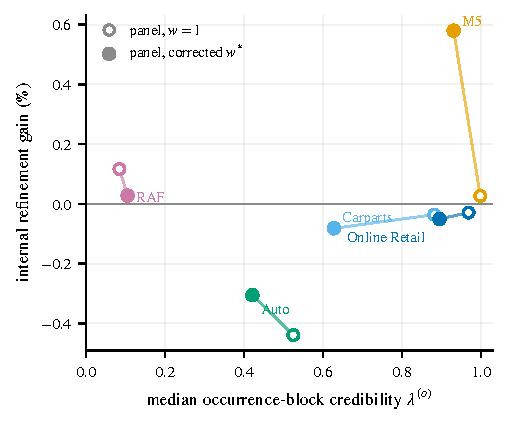
\includegraphics[width=\columnwidth]{figs/fig10b_refinement_leverage_occ.pdf}
\caption{\textbf{The simulated curves are an upper envelope that the real
panels do not reach.} Internal refinement gain (best refined structure
versus the global pool, validation SPL) against median credibility weight,
on the size block (top) and the occurrence block (bottom). Open markers
are $w{=}1$, filled markers the selected discount, and the connecting
segment is the movement forgetting induces. Grey curves are the controlled
panels of Section~\ref{sec:synthetic}, where the partition supplied is
correct by construction. % [ORIG 2026-09-13]
The grey curves pool the three separations of the
controlled grid; Figure~\ref{fig:separation} resolves them. Read against
the pooled envelope, every real panel lies below it at its own leverage.}
\label{fig:refinement-leverage}
\end{figure}


\paragraph{High leverage is an amplifier with no sign attached.}
The clearest illustration is RAF, which combines the highest size-block
leverage in the panel set ($\lambda^{(+)}=0.917$) with the lowest
occurrence leverage ($\lambda^{(o)}=0.106$), and loses $31.5\%$ of
external MAE to a learned partition. The two facts are one fact. The point
forecast is $\hat y_i=\hat\pi_i\exp(\hat\mu_i+\hat\sigma_i^2/2)$; when
$89\%$ of $\hat\pi_i$ comes from the group prior, replacing the group is
close to replacing the forecast. This is the empirical content of the
caveat attached to Proposition~\ref{prop:active}: persistent prior leverage
guarantees that the choice of target keeps mattering, not that a
particular target is good. Read together with the previous paragraph, low
leverage caps the upside and high leverage uncaps the downside, and
neither makes a learned partition worth using here.

\begin{table}[t]
\centering
\caption{Online Retail distributional ablation. Each row is an
independent hierarchical run; ``auto'' denotes its own internal discount
selection. The raw predictive law is used and lower is better. Full
point metrics are in Appendix Table~\ref{tab:ablation-full}.}
\label{tab:ablation}
\small
\begin{tabular*}{\columnwidth}{@{\extracolsep{\fill}}llrrr@{}}
\toprule
Pooling & Forget & SPL & SPL$_{90}$ & AIW\\
\midrule
global & off & 0.8899 & 1.5306 & 10.51\\
taxonomy & off & 0.8897 & 1.5299 & 10.56\\
learned & off & 0.8905 & 1.5336 & 10.79\\
global & auto ($.95$) & \secondbest{0.8849} & \secondbest{1.5268} & \best{9.25}\\
taxonomy & auto ($.95$) & \best{0.8846} & \best{1.5254} & 9.43\\
learned & auto ($.95$) & 0.8869 & 1.5343 & 10.69\\
\bottomrule
\end{tabular*}
\end{table}

\paragraph{What the ablation confirms.}
Table~\ref{tab:ablation} is the external counterpart on Online Retail: the
three pooling candidates differ by less than $0.1\%$ in mean SPL without
forgetting and by less than $0.3\%$ at the selected discount, matching the
internal picture. Discounting shows up
elsewhere, narrowing the global and taxonomy $80\%$ intervals by
$11$--$12\%$ while improving mean SPL by about half a percent; the full
ablation
(Appendix Table~\ref{tab:ablation-full}) shows it improves external MAE by
$3.5$--$4.0\%$ and slightly worsens RMSE. The cross-panel result in
Table~\ref{tab:prob} should therefore be attributed to the shared
hurdle-EB predictive law and to the temporal half of the selection, not to
a learned-partition gain. That is not a concession made after the fact:
the leverage diagnostic states the ceiling in advance, and
Figure~\ref{fig:refinement-leverage}\ shows we do not reach it.


\subsection{Pre-fit screen: protocol, metrics, and real-series transfer}
\label{app:room}

\begin{figure*}[t]
\centering
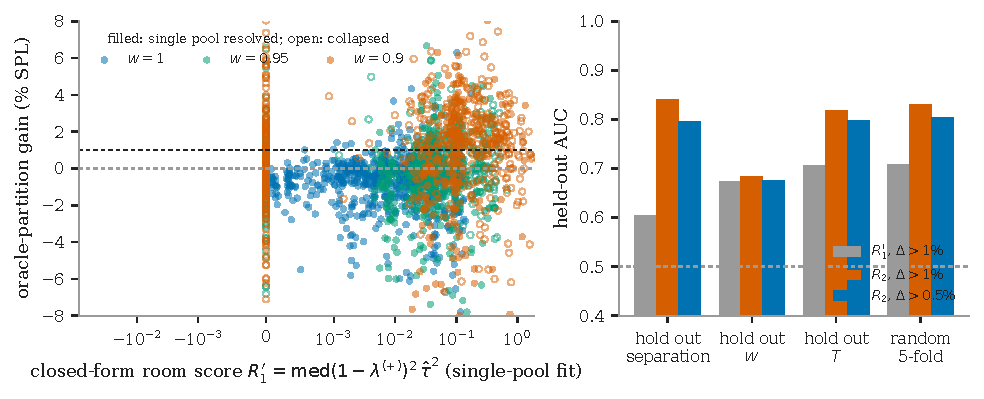
\includegraphics[width=0.96\textwidth]{figs/fig15_room_diagnostic.pdf}
\caption{\textbf{Screening for pooling room before any partition is
fitted.} Left: the closed-form score computed from the single-pool fit
against the oracle partition's realized gain on $2{,}700$ simulated
panels, colored by discount; open markers are panels whose single-pool
variance component collapsed. Right: held-out AUC for the event that the
oracle gain exceeds one percent (or half a percent), when whole
separation levels, discounts, or lengths are held out, or under random
folds; $R_1'$ is the closed-form score and $R_2$ a logistic screen on the
same fitting-window quantities.}
\label{fig:room}
\end{figure*}


\paragraph{Protocol.} The grid crosses separation $\{0,.25,.5,1,2\}$,
discount $\{1,.95,.90\}$, length $\{30,60,120\}$, occurrence mean
$\{.1,.25,.5\}$, items per group $\{20,60\}$, and balanced versus
$70/10/10/10$ group sizes, with four groups, $\tau^2=0.15$, $\sigma^2=1$,
occurrence separation scaled as $0.8\min(\mathrm{sep},1)$, five
replicates per cell, and seed 20260915. Per panel, only the single-pool
fit is used for features: median retained leverage on the size and
occurrence blocks, $\hat\tau^2$, the Beta concentration, the resolution
statistic, effective counts, and panel size. The target is the oracle
partition's paired pinball gain over the single pool (estimated
hyperparameters, true labels), which can be negative. The pre-registered
closed-form score $R_1$ used an unweighted mean of sampling variances
that is dominated by items whose discounted positive count approaches
zero; it has no screening power (AUC $0.45$--$0.64$) and is retained in
the released artifact. $R_1'$ replaces that term by the pool's own
weighted estimate $\hat\tau^2$; $R_2$ is a logistic regression on
$\log(1+\cdot)$ of the features, fitted on the training folds only. The
design, the amendments, and their order are recorded in
\texttt{docs/DESIGN\_room\_diagnostic.md}.

\begin{table}[t]
\centering
\caption{Held-out screening performance on the simulated grid for the
event that the oracle partition's gain exceeds one percent (base rate
$22\%$). Columns: AUC of the pre-registered $R_1$, of $R_1'$, and of the
logistic screen $R_2$ on all panels; the same for $R_1'$ and $R_2$ on the
panels whose single-pool variance component did not collapse; precision
and recall of $R_2$ at its best-$F_1$ threshold.}
\label{tab:room}
\small
\setlength{\tabcolsep}{3.5pt}
\begin{tabular}{lcccccc}
\toprule
 & \multicolumn{3}{c}{All panels} & \multicolumn{2}{c}{Resolved} & \\
\cmidrule(lr){2-4}\cmidrule(lr){5-6}
Held out & $R_1$ & $R_1'$ & $R_2$ & $R_1'$ & $R_2$ & $R_2$ P / R\\
\midrule
hold out a separation level & 0.45 & 0.60 & 0.84 & 0.72 & 0.85 & 0.54 / 0.77\\
hold out a discount & 0.64 & 0.67 & 0.68 & 0.66 & 0.68 & 0.51 / 0.49\\
hold out a length & 0.51 & 0.71 & 0.82 & 0.79 & 0.83 & 0.54 / 0.67\\
random 5-fold & 0.51 & 0.71 & 0.83 & 0.78 & 0.84 & 0.55 / 0.65\\
\bottomrule
\end{tabular}
\end{table}

\paragraph{Real-series transfer.} Online Retail, Carparts, and the
5{,}000-series M5 sample keep their zeros, noise, lengths, and scales; a
known partition is injected by multiplying every positive value of item
$i$ by $\exp(\delta_{g(i)})$ with symmetric offsets
$\{\pm0.5,\pm1.5\}\times\delta$, $\delta\in\{0,.25,.5,1,2\}$, over four
randomly assigned groups (three assignments), at the selected discount and
again at $w=0.90$. The oracle gain of the injected partition never exceeds
0.4\% on any panel: the single pool absorbs the injected
heterogeneity ($\hat\tau^2$ rises from $0.04$ to $5.1$ on Carparts as
$\delta$ goes from $0$ to $2$) and the median size-block credibility
rises toward one, so the items' own evidence, not the prior, carries the
forecast. $R_2$, fitted on the simulated grid and applied unchanged,
assigns every injected panel a probability below 0.17 of material
room (Figure~\ref{fig:room-transfer}). The transfer test therefore checks
the screen's rejections, not its detections; a real-series test of
detections would require panels whose items lack positive observations,
which is the short-history regime of Section~\ref{sec:pays}.

\begin{figure}[t]
\centering
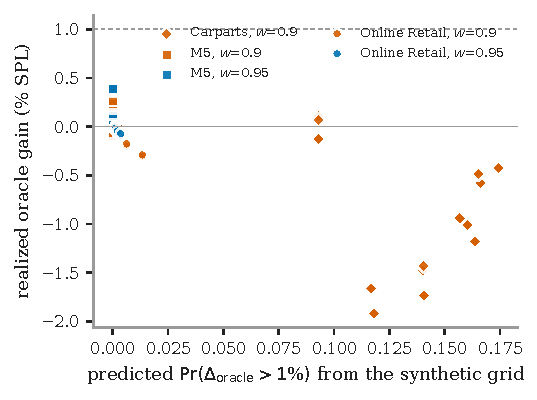
\includegraphics[width=0.9\linewidth]{figs/fig16_room_transfer.pdf}
\caption{Real-series transfer of the screen: predicted probability of
material room (from the simulated grid) against the realized oracle gain
of the injected partition, by panel and discount.}
\label{fig:room-transfer}
\end{figure}



\section{Additional results}\label{app:extra}

% -------------------------------------------------------------------------
\subsection{Point forecasting and horizon decomposition}
\label{app:point}

Table~\ref{tab:point} gives the complete point comparison retained for
continuity with the intermittent-demand literature. Rankings exclude the
deliberately degenerate Zero and Naive-last rows. \EBB{} takes six of
ten MAE/RMSSE cells and is top two on seven, but the result is not uniform:
classical methods retain several point-metric wins, and Zero attains the
lowest MAE on Online Retail, Carparts, and RAF. This is why the main text
uses point accuracy as a secondary diagnostic.

\begin{table*}[t]
\centering
\caption{Point forecasting across the five panels (lower is better;
bold best and underline second among non-degenerate methods). Degenerate
rows are shown as metric diagnostics and excluded from ranking.}
\label{tab:point}
\small
\setlength{\tabcolsep}{3.4pt}
\begin{tabular}{lcc@{\hspace{10pt}}cc@{\hspace{10pt}}cc@{\hspace{10pt}}cc@{\hspace{10pt}}cc}
\toprule
 & \multicolumn{2}{c}{Online Retail} & \multicolumn{2}{c}{M5} & \multicolumn{2}{c}{Auto} & \multicolumn{2}{c}{Carparts} & \multicolumn{2}{c}{RAF}\\
\cmidrule(lr){2-3}\cmidrule(lr){4-5}\cmidrule(lr){6-7}\cmidrule(lr){8-9}\cmidrule(lr){10-11}
Model & MAE & RMSSE & MAE & RMSSE & MAE & RMSSE & MAE & RMSSE & MAE & RMSSE\\
\midrule
CrostonClassic & 6.3294 & 5.1051 & 1.2345 & 2.3539 & 3.4056 & 1.1488 & 0.6792 & 1.0981 & 2.7315 & 1.6280\\
CrostonSBA & 6.1953 & 5.0692 & 1.2076 & 2.3517 & \secondbest{3.3325} & \secondbest{1.1451} & 0.6628 & 1.0935 & 2.6520 & 1.6272\\
TSB & \secondbest{5.5736} & 4.8031 & 1.2672 & 2.3612 & 3.6587 & 1.2066 & \best{0.5396} & 1.0156 & \best{2.1660} & 1.6570\\
TSB-tuned & 5.6318 & 4.7985 & \best{1.1932} & \secondbest{2.3137} & 3.3917 & 1.1452 & \best{0.5396} & 1.0156 & \secondbest{2.2447} & 1.6408\\
ADIDA & 5.6860 & \secondbest{4.7967} & 1.2274 & 2.3398 & 3.4079 & 1.1545 & 0.5556 & 1.0244 & 2.2977 & \secondbest{1.6245}\\
IMAPA & 5.7000 & 4.7970 & 1.2317 & 2.3280 & 3.4143 & 1.1555 & \secondbest{0.5524} & 1.0126 & 2.2850 & 1.6259\\
AutoARIMA & 6.5494 & 4.8175 & 1.2283 & 2.3169 & 3.4417 & 1.1745 & 0.5822 & \secondbest{1.0105} & 2.3153 & 1.6262\\
AutoTheta & 8.2862 & 4.8550 & 1.2988 & 2.3143 & 3.7490 & 1.2215 & 0.5704 & \best{0.9966} & 2.3687 & 1.6399\\
\midrule
Zero & 4.7549 & 4.8089 & 1.2995 & 2.4629 & 4.1444 & 1.4454 & 0.3867 & 1.0949 & 1.1717 & 1.6345\\
Naive-last & 6.0570 & 4.8324 & 1.3750 & 2.5450 & 4.3529 & 1.3818 & 0.5399 & 1.1408 & 1.8340 & 1.7644\\
\midrule
\EBB{} (ours) & \best{5.5325} & \best{4.7901} & \secondbest{1.2032} & \best{2.2938} & \best{3.2145} & \best{1.1374} & 0.5726 & 1.0120 & 2.3874 & \best{1.6245}\\
\bottomrule
\end{tabular}
\end{table*}

\begin{figure}[t]
\centering
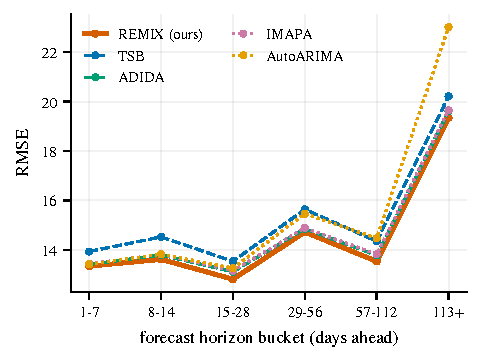
\includegraphics[width=0.93\linewidth]{figs/horizon_decomp.pdf}
\caption{Online Retail RMSE by fixed-origin forecast-horizon bucket.
\EBB{} is lowest in every bucket, so the aggregate result is not
created by averaging only over distant horizons. MAE differences among
the leading methods are within $1$--$2\%$ by bucket.}
\label{fig:horizon}
\end{figure}

The selected $(g,w)$ pairs are: Online Retail (global, $0.95$), M5
(mixture, $0.95$), Auto (global, $0.99$), Carparts (global, $0.90$), and
RAF (mixture, $0.997$). On three of the five panels the margins between
pooling structures on the internal validation surface are under a tenth
of a percent, so the structure component of these pairs should be read as
Section~\ref{sec:leverage} reads it: the selector avoids poor structural
corners, and no winner is announced where the surface does not resolve
one.

\subsection{Selector diagnostics}
\label{sec:selector-diagnostics}
\label{app:selector-diagnostics}

The selection surface is locally flat near its optimum: on Online Retail
the best seven candidates span all three pooling structures and lie within
$0.51\%$ of one another in validation SPL. Section~\ref{sec:leverage}
reports the credibility leverage and refinement gains that accompany each
selected pair, and Figure~\ref{fig:refinement-leverage} places them
against the controlled panels. The selector is useful for choosing a
discount and for avoiding poor structural corners; the winning pooling
structure on a panel whose candidates lie within a tenth of a percent
should not be read as a scientific taxonomy. Per-panel selection surfaces
are released with the code.

\begin{table*}[t]
\centering
\caption{Full Online Retail ablation corresponding to
Table~\ref{tab:ablation}. Each row is an independent run; ``auto'' denotes
its own internal discount selection. TSB has no native predictive
distribution. Lower is better.}
\label{tab:ablation-full}
\small
\setlength{\tabcolsep}{5.0pt}
\begin{tabular}{llrrrrrr}
\toprule
Pooling & Forget & MAE & RMSE & RMSSE & SPL & SPL$_{90}$ & AIW\\
\midrule
none (TSB) & fixed & 5.5736 & 18.7272 & 4.8031 & --- & --- & ---\\
global & off & 5.7623 & \best{17.6892} & \best{4.7851} & 0.8899 & 1.5306 & 10.51\\
taxonomy & off & 5.7663 & \secondbest{17.6930} & \secondbest{4.7875} & 0.8897 & 1.5299 & 10.56\\
learned & off & 5.8126 & 17.7064 & 4.7876 & 0.8905 & 1.5336 & 10.79\\
global & auto ($.95$) & \best{5.5325} & 17.8386 & 4.7901 & \secondbest{0.8849} & \secondbest{1.5268} & \best{9.25}\\
taxonomy & auto ($.95$) & \secondbest{5.5624} & 17.8421 & 4.7897 & \best{0.8846} & \best{1.5254} & 9.43\\
learned & auto ($.95$) & 5.6925 & 17.8765 & 4.7902 & 0.8869 & 1.5343 & 10.69\\
\bottomrule
\end{tabular}
\end{table*}

\subsection{Walk-forward point results and protocol}
\label{app:walkforward}

\begin{table}[t]
\centering
\caption{Online Retail point forecasting under strict seven-day
walk-forward updates. The hierarchical rows differ in their
initialization discount and pooling structure.}
\label{tab:walkforward}
\small
\setlength{\tabcolsep}{5pt}
\begin{tabular}{lccc}
\toprule
Model & MAE & RMSE & RMSSE\\
\midrule
CrostonClassic & 5.692 & 16.937 & 4.854\\
CrostonSBA & 5.586 & 16.931 & 4.836\\
TSB & 5.434 & 17.754 & 4.815\\
ADIDA & \best{5.320} & \best{16.728} & \secondbest{4.637}\\
IMAPA & \secondbest{5.332} & \secondbest{16.745} & \best{4.632}\\
AutoARIMA & 5.482 & 16.904 & 5.105\\
AutoTheta & 5.394 & 16.836 & 4.735\\
\midrule
Stationary hierarchy ($w=1$) & 5.586 & 17.260 & 4.725\\
Forgetting hierarchy (tax., $.95$) & 5.411 & 17.059 & 4.682\\
\EBB{} (selected global, $.95$) & 5.421 & 17.188 & 4.696\\
\bottomrule
\end{tabular}
\end{table}

\begin{table*}[t]
\centering
\caption{Full Online Retail walk-forward SPL at all five quantiles and on average,
with marginal (Cov@80) and positive-demand (Cov$^{+}$@80) coverage and
average interval width (AIW). CP and ACI wrappers refit each of the 36 seven-day blocks; AutoARIMA, AutoTheta, iETS, and TweedieGP refit every four blocks; \EBB{} updates sufficient statistics each block. The zero row is excluded from ranking.}
\label{tab:wfprob-full}
\small
\setlength{\tabcolsep}{4.2pt}
\begin{tabular}{lrrrrrrrrr}
\toprule
Model & q10 & q25 & q50 & q75 & q90 & Mean & Cov@80 & Cov$^{+}$@80 & AIW\\
\midrule
AutoARIMA & 0.259 & 0.572 & 1.197 & 1.763 & 1.522 & 1.063 & 0.933 & 0.762 & 16.58\\
AutoTheta & 0.233 & 0.584 & 1.276 & 1.717 & 1.484 & 1.059 & 0.931 & 0.765 & 16.43\\
iETS & 0.236 & 0.505 & 1.302 & 1.562 & 1.940 & 1.109 & 0.598 & 0.166 & 19.74\\
CP-Croston & 0.341 & 0.778 & 1.364 & 1.745 & 2.632 & 1.372 & 0.793 & 0.478 & 5.66\\
CP-SBA & 0.334 & 0.762 & 1.343 & 1.725 & 2.722 & 1.377 & 0.793 & 0.481 & 5.75\\
CP-TSB & 0.451 & 0.899 & 1.289 & 1.385 & 2.842 & 1.373 & 0.795 & 0.468 & 5.71\\
CP-ADIDA & 0.277 & 0.627 & 1.050 & \secondbest{1.319} & 2.514 & 1.158 & 0.791 & 0.473 & 5.47\\
CP-IMAPA & 0.292 & 0.660 & 1.083 & 1.329 & 2.522 & 1.177 & 0.791 & 0.471 & 5.47\\
ACI-ADIDA & 0.186 & 0.468 & \best{0.909} & 1.324 & 1.668 & 0.911 & 0.904 & 0.646 & 19.67\\
ACI-TSB & 0.189 & 0.482 & 0.948 & 1.384 & 1.710 & 0.943 & 0.903 & 0.641 & 21.21\\
TweedieGP & \secondbest{0.183} & \secondbest{0.458} & 0.917 & 1.326 & \best{1.379} & \best{0.853} & 0.924 & 0.709 & 13.03\\
Zero (diagnostic) & 0.183 & 0.458 & 0.916 & 1.374 & 1.649 & 0.916 & 0.740 & 0.000 & 0.00\\
\midrule
\EBB{} & 0.183 & 0.458 & \secondbest{0.910} & \best{1.319} & \secondbest{1.400} & \secondbest{0.854} & 0.901 & 0.621 & 10.31\\
ACI-\EBB{} & \best{0.183} & \best{0.458} & 0.915 & 1.423 & 1.562 & 0.908 & 0.913 & 0.665 & 19.55\\
\EBB{} (rule) & 0.183 & 0.458 & 0.910 & 1.319 & 1.400 & 0.854 & 0.901 & 0.621 & 10.31\\
\bottomrule
\end{tabular}
\end{table*}

\begin{table*}[t]
\centering
\caption{Full Carparts walk-forward SPL at all five quantiles and on average,
with marginal (Cov@80) and positive-demand (Cov$^{+}$@80) coverage and
average interval width (AIW). Every baseline refits each of the six monthly blocks; \EBB{} updates sufficient statistics. The zero row is excluded from ranking.}
\label{tab:wf-carparts-full}
\small
\setlength{\tabcolsep}{4.2pt}
\begin{tabular}{lrrrrrrrrr}
\toprule
Model & q10 & q25 & q50 & q75 & q90 & Mean & Cov@80 & Cov$^{+}$@80 & AIW\\
\midrule
AutoARIMA & 0.150 & 0.282 & 0.537 & 0.643 & 0.484 & 0.419 & 0.886 & 0.620 & 1.63\\
AutoTheta & 0.120 & 0.253 & 0.523 & 0.657 & 0.474 & 0.406 & 0.902 & 0.678 & 1.80\\
iETS & 0.272 & 0.368 & 0.493 & 0.532 & 0.515 & 0.436 & 0.442 & 0.411 & 1.17\\
CP-Croston & 0.099 & 0.245 & 0.480 & 0.614 & 0.539 & 0.395 & 0.847 & 0.580 & 1.39\\
CP-SBA & 0.098 & 0.242 & 0.475 & 0.611 & 0.538 & 0.393 & 0.847 & 0.581 & 1.37\\
CP-TSB & 0.141 & 0.301 & 0.487 & 0.513 & 0.476 & 0.384 & 0.834 & 0.551 & 1.27\\
CP-ADIDA & 0.096 & 0.230 & 0.411 & 0.529 & 0.488 & 0.351 & 0.829 & 0.593 & 1.28\\
CP-IMAPA & 0.101 & 0.235 & 0.413 & 0.518 & 0.479 & 0.349 & 0.830 & 0.581 & 1.27\\
ACI-ADIDA & 0.088 & 0.221 & 0.406 & 0.517 & 0.477 & 0.342 & 0.870 & 0.604 & 1.38\\
TweedieGP & 0.075 & 0.188 & 0.375 & 0.490 & \best{0.433} & \best{0.312} & 0.931 & 0.662 & 1.46\\
Zero (diagnostic) & 0.075 & 0.187 & 0.374 & 0.560 & 0.672 & 0.374 & 0.795 & 0.000 & 0.00\\
\midrule
\EBB{} & \secondbest{0.075} & \secondbest{0.187} & \secondbest{0.372} & \secondbest{0.481} & 0.458 & 0.315 & 0.932 & 0.669 & 1.42\\
ACI-\EBB{} & \best{0.075} & \best{0.187} & \best{0.371} & \best{0.480} & \secondbest{0.452} & \secondbest{0.313} & 0.934 & 0.676 & 1.41\\
\EBB{} (rule) & 0.075 & 0.187 & 0.372 & 0.481 & 0.458 & 0.315 & 0.932 & 0.669 & 1.42\\
\bottomrule
\end{tabular}
\end{table*}

\begin{table*}[t]
\centering
\caption{Full Auto walk-forward SPL at all five quantiles and on average,
with marginal (Cov@80) and positive-demand (Cov$^{+}$@80) coverage and
average interval width (AIW). Every baseline refits each of the six monthly blocks; \EBB{} updates sufficient statistics. The zero row is excluded from ranking.}
\label{tab:wf-auto-full}
\small
\setlength{\tabcolsep}{4.2pt}
\begin{tabular}{lrrrrrrrrr}
\toprule
Model & q10 & q25 & q50 & q75 & q90 & Mean & Cov@80 & Cov$^{+}$@80 & AIW\\
\midrule
AutoARIMA & 0.141 & 0.313 & 0.447 & 0.405 & 0.263 & 0.314 & 0.778 & 0.799 & 8.73\\
AutoTheta & 0.152 & 0.320 & 0.460 & 0.418 & 0.262 & 0.322 & 0.780 & 0.825 & 9.64\\
iETS & 0.172 & 0.312 & 0.435 & 0.423 & 0.301 & 0.329 & 0.564 & 0.690 & 7.33\\
CP-Croston & 0.148 & 0.307 & 0.437 & 0.402 & 0.296 & 0.318 & 0.801 & 0.802 & 5.97\\
CP-SBA & 0.146 & 0.304 & 0.434 & 0.404 & 0.301 & 0.318 & 0.800 & 0.803 & 6.01\\
CP-TSB & 0.155 & 0.321 & 0.458 & 0.414 & 0.301 & 0.330 & 0.808 & 0.799 & 5.97\\
CP-ADIDA & 0.149 & 0.307 & 0.437 & 0.400 & 0.295 & 0.318 & 0.802 & 0.802 & 5.92\\
CP-IMAPA & 0.149 & 0.307 & 0.437 & 0.400 & 0.295 & 0.318 & 0.802 & 0.802 & 5.92\\
ACI-ADIDA & 0.139 & 0.305 & 0.438 & 0.401 & 0.290 & 0.315 & 0.830 & 0.822 & 6.74\\
TweedieGP & 0.122 & 0.279 & \secondbest{0.418} & \best{0.389} & \best{0.254} & 0.292 & 0.834 & 0.828 & 8.81\\
Zero (diagnostic) & 0.112 & 0.281 & 0.561 & 0.842 & 1.010 & 0.561 & 0.262 & 0.000 & 0.00\\
\midrule
\EBB{} & \best{0.112} & \secondbest{0.275} & 0.418 & 0.393 & 0.256 & \secondbest{0.291} & 0.906 & 0.873 & 9.17\\
ACI-\EBB{} & \secondbest{0.113} & \best{0.275} & \best{0.416} & \secondbest{0.391} & \secondbest{0.256} & \best{0.290} & 0.905 & 0.876 & 9.41\\
\EBB{} (rule) & 0.113 & 0.275 & 0.416 & 0.391 & 0.256 & 0.290 & 0.905 & 0.876 & 9.41\\
\bottomrule
\end{tabular}
\end{table*}

\begin{table*}[t]
\centering
\caption{Full RAF walk-forward SPL at all five quantiles and on average,
with marginal (Cov@80) and positive-demand (Cov$^{+}$@80) coverage and
average interval width (AIW). Every baseline refits each of the twelve monthly blocks; \EBB{} updates sufficient statistics. The zero row is excluded from ranking.}
\label{tab:wf-raf-full}
\small
\setlength{\tabcolsep}{4.2pt}
\begin{tabular}{lrrrrrrrrr}
\toprule
Model & q10 & q25 & q50 & q75 & q90 & Mean & Cov@80 & Cov$^{+}$@80 & AIW\\
\midrule
AutoARIMA & 0.066 & 0.151 & 0.490 & 0.742 & 0.592 & 0.408 & 0.944 & 0.352 & 8.76\\
AutoTheta & 0.066 & 0.158 & 0.497 & 0.809 & 0.623 & 0.431 & 0.948 & 0.409 & 10.03\\
iETS & 0.220 & 0.270 & 0.353 & 0.435 & 0.490 & 0.354 & 0.495 & 0.019 & 0.53\\
CP-Croston & 0.090 & 0.216 & 0.381 & 0.471 & 0.492 & 0.330 & 0.828 & 0.045 & 1.03\\
CP-SBA & 0.088 & 0.212 & 0.375 & 0.468 & 0.491 & 0.327 & 0.828 & 0.041 & 0.98\\
CP-TSB & 0.160 & 0.317 & 0.462 & 0.488 & 0.494 & 0.384 & 0.836 & 0.025 & 0.37\\
CP-ADIDA & 0.078 & 0.187 & 0.343 & 0.449 & \secondbest{0.489} & 0.309 & 0.823 & 0.021 & 0.72\\
CP-IMAPA & 0.082 & 0.192 & 0.348 & 0.452 & 0.490 & 0.313 & 0.824 & 0.019 & 0.69\\
ACI-ADIDA & 0.057 & 0.154 & 0.326 & 0.446 & 0.560 & 0.308 & 0.909 & 0.083 & 1.85\\
TweedieGP & 0.053 & 0.134 & 0.270 & 0.417 & 0.526 & 0.280 & 0.935 & 0.198 & 4.07\\
Zero (diagnostic) & 0.053 & 0.134 & 0.267 & 0.400 & 0.480 & 0.267 & 0.919 & 0.000 & 0.00\\
\midrule
\EBB{} & \secondbest{0.053} & \secondbest{0.134} & \secondbest{0.267} & \best{0.400} & \best{0.486} & \best{0.268} & 0.922 & 0.041 & 0.95\\
ACI-\EBB{} & \best{0.053} & \best{0.134} & \best{0.267} & \secondbest{0.401} & 0.517 & \secondbest{0.274} & 0.927 & 0.101 & 2.07\\
\EBB{} (rule) & 0.053 & 0.134 & 0.267 & 0.400 & 0.486 & 0.268 & 0.922 & 0.041 & 0.95\\
\bottomrule
\end{tabular}
\end{table*}

\begin{table*}[t]
\centering
\caption{Full M5 walk-forward SPL at all five quantiles and on average,
with marginal (Cov@80) and positive-demand (Cov$^{+}$@80) coverage and
average interval width (AIW). Static CP wrappers and ACI-ADIDA refit each of the 93 seven-day blocks on the 5{,}000-series sample; AutoARIMA, AutoTheta, iETS, and TweedieGP were not run under this protocol on cost grounds; \EBB{} updates sufficient statistics each block. The zero row is excluded from ranking.}
\label{tab:wf-m5-full}
\small
\setlength{\tabcolsep}{4.2pt}
\begin{tabular}{lrrrrrrrrr}
\toprule
Model & q10 & q25 & q50 & q75 & q90 & Mean & Cov@80 & Cov$^{+}$@80 & AIW\\
\midrule
CP-Croston & 0.502 & 1.150 & 1.917 & 2.343 & 1.923 & 1.567 & 0.812 & 0.679 & 2.26\\
CP-SBA & 0.495 & 1.137 & 1.909 & 2.385 & 1.956 & 1.576 & 0.812 & 0.684 & 2.28\\
CP-TSB & 0.531 & 1.263 & 2.094 & 2.377 & 2.042 & 1.662 & 0.831 & 0.685 & 2.37\\
CP-ADIDA & 0.479 & 1.108 & 1.889 & 2.330 & 1.963 & 1.554 & 0.827 & 0.690 & 2.28\\
CP-IMAPA & 0.480 & 1.110 & 1.889 & 2.301 & 1.949 & 1.546 & 0.828 & 0.691 & 2.28\\
ACI-ADIDA & 0.402 & \secondbest{0.960} & \best{1.718} & \secondbest{2.211} & \secondbest{1.806} & \secondbest{1.419} & 0.883 & 0.718 & 3.48\\
Zero (diagnostic) & 0.392 & 0.980 & 1.959 & 2.938 & 3.526 & 1.959 & 0.606 & 0.000 & 0.00\\
\midrule
\EBB{} & \secondbest{0.391} & 0.967 & 1.852 & 2.336 & 1.880 & 1.485 & 0.875 & 0.690 & 2.77\\
ACI-\EBB{} & \best{0.389} & \best{0.951} & \secondbest{1.768} & \best{2.140} & \best{1.644} & \best{1.379} & 0.891 & 0.730 & 3.00\\
\EBB{} (rule) & 0.389 & 0.951 & 1.768 & 2.140 & 1.644 & 1.379 & 0.891 & 0.730 & 3.00\\
\bottomrule
\end{tabular}
\end{table*}

\begin{table*}[t]
\centering
\caption{Per-panel mean-SPL regret (percent) to the best non-degenerate
method on that panel, under the fixed-origin and walk-forward protocols.
Zero regret marks the panel leader. Dashes mark methods not run under
that protocol on that panel.}
\label{tab:regret-full}
\small
\setlength{\tabcolsep}{4.2pt}
\begin{tabular}{lrrrrrrrrrr}
\toprule
 & \multicolumn{5}{c}{Fixed origin} & \multicolumn{5}{c}{Walk-forward}\\
\cmidrule(lr){2-6}\cmidrule(lr){7-11}
Method & OR & Carparts & Auto & RAF & M5 & OR & Carparts & Auto & RAF & M5\\
\midrule
AutoARIMA & 13.8 & 27.1 & 8.6 & 50.0 & 10.4 & 24.6 & 34.4 & 8.2 & 52.3 & ---\\
AutoTheta & 13.7 & 22.1 & 15.9 & 53.1 & 10.6 & 24.2 & 30.0 & 11.1 & 60.7 & ---\\
Tweedie-GLM & 29.8 & 48.6 & 9.7 & 16.5 & 150.8 & --- & --- & --- & --- & ---\\
iETS & 11.3 & 41.9 & 17.4 & 30.4 & 25.0 & 30.1 & 39.8 & 13.3 & 31.9 & ---\\
CP-Croston & 75.3 & 24.8 & 11.0 & 24.0 & 4.2 & 60.9 & 26.7 & 9.7 & 23.1 & 13.7\\
CP-SBA & 75.1 & 23.9 & 10.9 & 22.8 & 4.4 & 61.5 & 25.9 & 9.5 & 21.9 & 14.4\\
CP-TSB & 32.8 & 17.7 & 17.8 & 42.3 & 15.8 & 61.1 & 22.9 & 13.7 & 43.3 & 20.5\\
CP-ADIDA & 27.1 & 11.1 & 11.5 & 15.6 & 5.7 & 35.8 & 12.4 & 9.4 & 15.4 & 12.7\\
CP-IMAPA & 27.5 & 10.8 & 11.6 & 16.3 & 5.9 & 38.1 & 11.9 & 9.5 & 16.6 & 12.1\\
ACI-ADIDA & --- & --- & --- & --- & --- & 6.8 & 9.5 & 8.5 & 15.1 & 3.0\\
TweedieGP & 0.0 & 0.0 & 1.6 & 3.1 & 0.0 & 0.0 & 0.0 & 0.8 & 4.5 & ---\\
\midrule
\EBB{} & 0.0 & 0.5 & 0.0 & 0.0 & 3.0 & 0.2 & 0.8 & 0.3 & 0.0 & 7.7\\
ACI-\EBB{} & --- & --- & --- & --- & --- & 6.5 & 0.2 & 0.0 & 2.3 & 0.0\\
\EBB{} (rule) & --- & --- & --- & --- & --- & 0.2 & 0.8 & 0.0 & 0.0 & 0.0\\
\bottomrule
\end{tabular}
\end{table*}

\begin{table*}[t]
\centering
\caption{Short-history scaling: initialization window truncated to its
last $L$ observations per series (evaluation span unchanged; SPL scale
from the full window). Median credibility weights at the audited discount,
mean SPL of \EBB{}, TweedieGP, and CP-ADIDA, and \EBB{}'s advantage over
TweedieGP. Mixture labels are re-learned on the truncated window.}
\label{tab:coldstart}
\small
\setlength{\tabcolsep}{4.5pt}
\begin{tabular}{llrrrrrrr}
\toprule
Panel & $L$ & median $n$ & $\lambda^{(o)}$ & $\lambda^{(+)}$ & \EBB{} & TweedieGP & CP-ADIDA & Adv.\ (\%)\\
\midrule
Online Retail & 14 & 14 & 0.823 & 0.405 & 0.8894 & 0.8920 & 1.0106 & +0.3\\
 & 28 & 28 & 0.870 & 0.506 & 0.8862 & 0.8879 & 1.1519 & +0.2\\
 & 56 & 56 & 0.893 & 0.546 & 0.8852 & 0.8859 & 1.1247 & +0.1\\
 & full & 119 & 0.895 & 0.553 & 0.8849 & 0.8845 & 1.1239 & -0.0\\
\addlinespace
M5 & 28 & 28 & 0.910 & 0.812 & 1.6925 & 1.6626 & 1.7182 & -1.8\\
 & 56 & 56 & 0.928 & 0.839 & 1.6645 & 1.6774 & 1.7082 & +0.8\\
 & 112 & 112 & 0.930 & 0.844 & 1.6697 & 1.6558 & 1.6912 & -0.8\\
 & 224 & 224 & 0.931 & 0.842 & 1.6637 & 1.5995 & 1.7092 & -4.0\\
 & 448 & 448 & 0.931 & 0.842 & 1.6670 & 1.6063 & 1.7024 & -3.8\\
 & full & 1294 & 0.931 & 0.841 & 1.6707 & 1.6228 & 1.7150 & -3.0\\
\addlinespace
Auto & 6 & 6 & 0.278 & 0.867 & 0.3009 & 0.3221 & 0.3363 & +6.6\\
 & 12 & 12 & 0.377 & 0.920 & 0.2948 & 0.3017 & 0.3317 & +2.3\\
 & full & 18 & 0.421 & 0.940 & 0.2937 & 0.2985 & 0.3275 & +1.6\\
\addlinespace
Carparts & 6 & 6 & 0.585 & 0.180 & 0.3199 & 0.3279 & 0.3858 & +2.4\\
 & 12 & 12 & 0.560 & 0.231 & 0.3197 & 0.3173 & 0.3628 & -0.8\\
 & 24 & 24 & 0.596 & 0.245 & 0.3206 & 0.3145 & 0.3585 & -1.9\\
 & full & 45 & 0.628 & 0.224 & 0.3229 & 0.3214 & 0.3571 & -0.5\\
\addlinespace
RAF & 6 & 6 & 0.037 & 0.000 & 0.2730 & 0.3079 & 0.4071 & +11.3\\
 & 12 & 12 & 0.075 & 0.682 & 0.2696 & 0.2811 & 0.3506 & +4.1\\
 & 24 & 24 & 0.135 & 0.790 & 0.2669 & 0.2788 & 0.3208 & +4.3\\
 & 48 & 48 & 0.152 & 0.891 & 0.2674 & 0.2769 & 0.3141 & +3.4\\
 & full & 72 & 0.106 & 0.917 & 0.2680 & 0.2763 & 0.3097 & +3.0\\
\bottomrule
\end{tabular}
\end{table*}

% [ORIG 2026-09-06]
% ORIG| % [2026-09-06 STALE] With TweedieGP in the walk-forward roster this paragraph no longer holds on
% ORIG| % Online Retail (TweedieGP takes the mean 0.8526 vs 0.8540 and q90 1.3791 vs 1.4002; EBB keeps q75)
% ORIG| % or Carparts (TweedieGP takes the mean and q90; EBB keeps q10-q75). Auto/RAF/M5 tables are new.
% ORIG| \EBB{} applies the selected discount once to the initialization
% ORIG| sufficient statistics and then accumulates revealed blocks without
% ORIG| compounding it. On Online Retail, ACI-ADIDA improves the static conformal
% ORIG| wrapper substantially and wins q50 by a hair, but \EBB{} takes every
% ORIG| other quantile, the mean, and q90 by a clear margin. On Carparts the
% ORIG| first two quantiles saturate at zero and the discriminating gains occur
% ORIG| from the median up.
\EBB{} applies the selected discount once to the initialization
sufficient statistics and then accumulates revealed blocks without
compounding it. On Online Retail, ACI-ADIDA improves the static conformal
wrapper substantially and wins q50 by a hair; TweedieGP takes the mean
and q90, and \EBB{} takes q75 and is second elsewhere. On Carparts the
first two quantiles saturate at zero, \EBB{} leads from q10 through q75,
and TweedieGP takes q90 and the mean. On Auto \EBB{} leads q10, q25, and
the mean while TweedieGP leads q50 through q90; on RAF \EBB{} leads every
% [ORIG 2026-09-07]
% ORIG| quantile, coinciding with the zero forecast through q75; on M5 ACI-ADIDA
% ORIG| leads q25 through q90 and the mean, and \EBB{} leads q10.
quantile, coinciding with the zero forecast through q75; on M5 ACI-\EBB{}
leads every quantile from q25 up and the mean, ACI-ADIDA is second, and
uncalibrated \EBB{} leads q10. ACI-\EBB{} improves on \EBB{} on M5, Auto,
and Carparts and degrades it on Online Retail and RAF
(Table~\ref{tab:wf-significance}).
Table~\ref{tab:regret-full} gives the per-panel regrets behind
Table~\ref{tab:regret}. Re-running joint selection at every block is not
evaluated.


\subsection{Three model-side remedies that do not close the gap}
\label{app:negative}

Section~\ref{sec:main-results} locates the remaining shortfall to
TweedieGP on Online Retail, Carparts, and M5. Three remedies within the
\EBB{} family are the obvious candidates: a heavier-tailed positive-size
law, an item-specific forgetting rate, and a separate forgetting rate for
the occurrence block. Both were evaluated on the
fixed-origin protocol with the audited pooling structure and, for the
size law, the identical fitted posterior; neither changes any panel's
leader.

\textbf{Predictive-law shape.} Table~\ref{tab:shape} replaces the
log-normal predictive law of \eqref{eq:predictive-law} by log-$t$,
moment-matched Gamma, and inflated-scale alternatives computed from the
same item posteriors. Mean SPL moves by at most $0.003$ on every panel and
in no case reaches TweedieGP.

\begin{table}[t]
\centering
\caption{Mean SPL of alternative positive-size predictive laws computed
from the same fitted \EBB{} posterior (single fit, no bootstrap averaging),
against TweedieGP.}
\label{tab:shape}
\small
\setlength{\tabcolsep}{3.5pt}
\begin{tabular}{lrrrrr}
\toprule
Size law & OR & Carparts & Auto & RAF & M5\\
\midrule
log-normal (released) & 0.8849 & 0.3230 & 0.2937 & 0.2681 & 1.6730\\
log-$t$, $\nu{=}10$ & 0.8849 & 0.3228 & 0.2936 & 0.2680 & 1.6735\\
log-$t$, $\nu{=}5$ & 0.8850 & 0.3226 & 0.2940 & 0.2678 & 1.6744\\
Gamma (moment-matched) & 0.8878 & 0.3227 & 0.2937 & 0.2673 & 1.6735\\
\midrule
TweedieGP & 0.8845 & 0.3214 & 0.2985 & 0.2763 & 1.6228\\
\bottomrule
\end{tabular}
\end{table}

\textbf{Item-specific forgetting.} Each item receives its own discount
$w_i$, chosen on an inner chronological split of the fitting head by
minimizing $n_i^{V}R_i(w)+\kappa\bar R(w)$, where $R_i$ is the item's
validation pinball curve over the grid of Section~\ref{sec:select},
$\bar R$ the panel average, and $\kappa$ an empirical-Bayes shrinkage
strength selected on the outer validation tail;
$\kappa{=}\infty$ recovers the panel-wide $w^{\star}$ and $\kappa{=}0$
leaves each item unshrunk. Table~\ref{tab:peritem} reports the result.
The pre-registered adoption criterion (improve Online Retail or M5 by at
least $1\%$ without degrading Auto or RAF by more than $0.3\%$, and
either recover Online Retail from TweedieGP or bring M5 within $1.5\%$ of
it) fails on its second clause: M5 improves by $1.15\%$ but remains
$1.8\%$ behind, and Online Retail is unchanged. Unshrunk selection
($\kappa{=}0$) is markedly worse on M5, so the shrinkage is necessary; the
selected $\kappa$ is interior on four panels. The per-item option is
retained in the released code but is not used in any reported result.

\begin{table*}[t]
\centering
\caption{Item-specific forgetting rates with shrinkage strength $\kappa$
selected on the outer validation tail. $w^{\star}$ is the panel-wide
discount; ``share $<w^{\star}$'' is the fraction of items that selected
faster forgetting than the panel rate; $\kappa{=}\infty$ and $\kappa{=}0$
give the fully shrunk and unshrunk endpoints. External mean SPL,
$B{=}20$.}
\label{tab:peritem}
\small
\setlength{\tabcolsep}{4pt}
\begin{tabular}{lrrrrrrrrr}
\toprule
Panel & $w^{\star}$ & Scalar & $\kappa^{\star}$ & Per-item & $\Delta$ (\%) & share $<w^{\star}$ & $\kappa{=}\infty$ & $\kappa{=}0$ & TweedieGP\\
\midrule
Online Retail & 0.95 & 0.8849 & 10 & 0.8846 & -0.03 & 0.19 & 0.8849 & 0.8845 & 0.8845\\
Carparts & 0.9 & 0.3229 & $\infty$ & 0.3229 & +0.00 & 0.00 & 0.3229 & 0.3298 & 0.3214\\
Auto & 0.99 & 0.2937 & 30 & 0.2940 & +0.10 & 0.14 & 0.2942 & 0.2931 & 0.2985\\
RAF & 0.997 & 0.2680 & 100 & 0.2678 & -0.07 & 0.16 & 0.2680 & 0.2675 & 0.2763\\
M5 & 0.95 & 1.6707 & 3 & 1.6515 & -1.15 & 0.49 & 1.6751 & 1.8155 & 1.6228\\
\bottomrule
\end{tabular}
\end{table*}

\textbf{Separate occurrence forgetting.} The M5 shortfall sits in the
occurrence block (Section~\ref{sec:main-results}), and TSB itself smooths
occurrence and size with two constants, so a third remedy gives the
occurrence counts their own discount $w^{(o)}$ while the size statistics
keep the selected $w$. $w^{(o)}$ is chosen on the same 80/20 chronological
split and criterion as $w$, from a grid that contains the tied value.
Table~\ref{tab:occdisc} reports the result. The selector keeps the tied
rate on Online Retail, Auto, and RAF, moves M5 by $0.14\%$, and moves
Carparts by $0.77\%$ (to $0.3204$, marginally ahead of TweedieGP); the
pre-registered criterion of a $1\%$ gain on M5 is not met, so the single
rate is retained. A faster occurrence rate ($w^{(o)}{=}0.8$) removes every
zero q90 forecast on M5 and lowers q90 SPL from $2.476$ to $2.452$ without
changing the mean, which locates the M5 tail problem in occurrence
persistence rather than in the size law, but the selector does not choose
it and we do not override the selector.

\begin{table*}[t]
\centering
\caption{Separate occurrence discount $w^{(o)}$ with the size discount
fixed at the selected $w$; $w^{(o)\star}$ is chosen on the initialization
window's validation tail. External mean SPL ($B{=}20$) for the tied and
selected rates, the share of evaluation rows whose q90 forecast is exactly
zero, and TweedieGP for reference.}
\label{tab:occdisc}
\small
\setlength{\tabcolsep}{5pt}
\begin{tabular}{lccccccc}
\toprule
Panel & $w$ & $w^{(o)\star}$ & Tied & Selected & $\Delta$ (\%) & q90 $=0$ share & TweedieGP\\
\midrule
Online Retail & 0.95 & tied & 0.8849 & 0.8849 & +0.00 & 0.362 $\to$ 0.362 & 0.8845\\
M5 & 0.95 & 0.98 & 1.6707 & 1.6683 & -0.14 & 0.206 $\to$ 0.233 & 1.6228\\
Auto & 0.99 & tied & 0.2937 & 0.2937 & +0.00 & 0.000 $\to$ 0.000 & 0.2985\\
Carparts & 0.9 & 0.8 & 0.3229 & 0.3204 & -0.77 & 0.081 $\to$ 0.000 & 0.3214\\
RAF & 0.997 & tied & 0.2680 & 0.2680 & +0.00 & 0.279 $\to$ 0.279 & 0.2763\\
\bottomrule
\end{tabular}
\end{table*}

\subsection{Significance and interval diagnostics}
\label{sec:significance}

\begin{table}[t]
\centering
\caption{Per-series mean SPL paired tests: \EBB{} versus every
comparator on each panel, Holm-adjusted within panel (paired $t$ and
Wilcoxon signed-rank; the family includes TweedieGP on every
panel). Cells count comparators by outcome at the $5\%$ level; named
entries are the comparators for which \EBB{} is \emph{not}
significantly better.}
\label{tab:spl-significance}
\small
\setlength{\tabcolsep}{4.0pt}
\begin{tabular}{lcccl}
\toprule
Panel & Family & Sig.\ better & Sig.\ worse & Undecided\\
\midrule
Online Retail & 10 & 9 & 0 & TweedieGP\\
M5 & 10 & 5 & 1 (TweedieGP) & CP wrappers (4)\\
Auto & 10 & 10 & 0 & ---\\
Carparts & 10 & 9 & 0 & TweedieGP\\
RAF & 10 & 10 & 0 & ---\\
\bottomrule
\end{tabular}
\end{table}

\begin{table*}[t]
\centering
\caption{Walk-forward per-series paired tests, Holm-adjusted within each
(panel, reference) family; a comparison is significant when both the
paired $t$ and the Wilcoxon adjusted $p$ are below $0.05$. Families
contain every walk-forward method with stored per-series quantiles;
TweedieGP is not in the M5 family and the static conformal wrappers are
not in the Online Retail family.}
\label{tab:wf-significance}
\small
\setlength{\tabcolsep}{5pt}
\begin{tabular}{llcccl}
\toprule
Panel & Reference & Family & Sig.\ better & Sig.\ worse & Undecided\\
\midrule
Online Retail & \EBB{} & 7 & 6 & 0 & TweedieGP\\
Carparts & \EBB{} & 11 & 9 & 0 & ACI-\EBB{}, TweedieGP\\
Auto & \EBB{} & 11 & 9 & 0 & ACI-\EBB{}, TweedieGP\\
RAF & \EBB{} & 11 & 11 & 0 & ---\\
M5 & \EBB{} & 7 & 5 & 2 (ACI-ADIDA, ACI-\EBB{}) & ---\\
Online Retail & ACI-\EBB{} & 7 & 4 & 2 (\EBB{}, TweedieGP) & ACI-ADIDA\\
Carparts & ACI-\EBB{} & 11 & 9 & 0 & \EBB{}, TweedieGP\\
Auto & ACI-\EBB{} & 11 & 10 & 0 & TweedieGP\\
RAF & ACI-\EBB{} & 11 & 10 & 1 (\EBB{}) & ---\\
M5 & ACI-\EBB{} & 7 & 7 & 0 & ---\\
\bottomrule
\end{tabular}
\end{table*}

\begin{table*}[t]
\centering
\caption{Validation-tail rule for the calibration layer. On the 80/20
chronological split of the initialization window, \EBB{} is initialized on
the head (labels learned on the head only) and walked forward over the
tail with and without the adaptive conformal layer; the layer is applied
in deployment iff its tail scaled pinball ($q\in\{.5,.75,.9\}$) is lower.
External columns are the walk-forward means of Table~\ref{tab:wfprob};
``matches'' marks panels where the rule picks the ex-post better variant.}
\label{tab:aci-rule}
\small
\setlength{\tabcolsep}{5pt}
\begin{tabular}{lrrrlrrc}
\toprule
Panel & Tail blocks & Tail plain & Tail ACI & Choice & Ext.\ \EBB{} & Ext.\ ACI-\EBB{} & Matches\\
\midrule
Online Retail & 4 & 0.7382 & 0.7967 & plain & 0.8540 & 0.9082 & yes\\
M5 & 37 & 1.5686 & 1.4457 & ACI & 1.4851 & 1.3785 & yes\\
Auto & 3 & 0.3313 & 0.3304 & ACI & 0.2910 & 0.2901 & yes\\
Carparts & 9 & 0.8975 & 0.9061 & plain & 0.3145 & 0.3128 & no\\
RAF & 14 & 0.9846 & 1.0081 & plain & 0.2681 & 0.2743 & yes\\
\bottomrule
\end{tabular}
\end{table*}

\begin{table}[t]
\centering
\caption{Paired per-series MAE tests on Online Retail: \EBB{} versus
each alternative. Negative mean differences favor \EBB{}; $p$-values
are Holm-adjusted.}
\label{tab:significance}
\small
\setlength{\tabcolsep}{5pt}
\begin{tabular}{lccc}
\toprule
vs. & Mean diff & $p_t$ & $p_{\mathrm{Wilcoxon}}$\\
\midrule
Stationary hierarchy & $-0.165$ & $<10^{-29}$ & $<10^{-11}$\\
TSB & $-0.040$ & $0.532$ & $<10^{-155}$\\
TSB-tuned & $-0.090$ & $0.086$ & $<10^{-72}$\\
ADIDA & $-0.036$ & $0.359$ & $<10^{-88}$\\
IMAPA & $-0.049$ & $0.281$ & $<10^{-97}$\\
CrostonSBA & $-0.872$ & $<10^{-26}$ & $<10^{-59}$\\
AutoARIMA & $-0.891$ & $<10^{-14}$ & $<10^{-12}$\\
AutoTheta & $-2.644$ & $<10^{-81}$ & $<10^{-104}$\\
\bottomrule
\end{tabular}
\end{table}

\begin{table}[t]
\centering
\caption{Raw \EBB{} interval quality across panels at nominal $80\%$
coverage. No post-hoc calibration is used.}
\label{tab:coverage}
\small
\setlength{\tabcolsep}{4.6pt}
\begin{tabular}{lccccc}
\toprule
 & OR & M5 & Auto & Carparts & RAF\\
\midrule
Coverage@80 & 0.892 & 0.846 & 0.907 & 0.931 & 0.921\\
AIW@80 & 9.25 & 2.81 & 9.21 & 1.47 & 0.94\\
\bottomrule
\end{tabular}
\end{table}

Table~\ref{tab:spl-significance} tests the headline metric directly:
per-series mean SPL, \EBB{} against every comparator of
Table~\ref{tab:prob}, with paired $t$ and Wilcoxon signed-rank tests
Holm-adjusted within each panel and a comparison counted as decided only
when both adjusted tests agree at the $5\%$ level. \EBB{} is
significantly better in 43 of the 50 panel--comparator pairs,
significantly worse in one (TweedieGP on M5, adjusted $p=0.003$ and
$0.035$), and undecided in six. On M5 the mean difference favors
\EBB{} against all four conformal wrappers but the paired $t$ does not
reach significance after correction (the Wilcoxon strongly rejects
symmetry, so the per-series differences are systematic but
heavy-tailed); on Carparts neither \EBB{} nor TweedieGP separates from
the other (adjusted $p\ge0.50$ both ways), consistent with the
half-percent aggregate margin between them; and on Online Retail
TweedieGP is ahead by $0.04\%$ in mean SPL with the paired $t$ at
$p=0.71$. \EBB{} is significantly better than TweedieGP on Auto and
RAF.

The paired MAE tests support a systematic improvement over the stationary
hierarchy. Against TSB, tuned TSB, ADIDA, and IMAPA, mean MAE favors
\EBB{} but the adjusted paired $t$-tests are not significant; the
Wilcoxon tests reverse because those methods win on the typical series
while \EBB{} reduces the difficult-series tail. On per-series RMSE,
both adjusted tests favor \EBB{} against every comparator at $p<0.05$.
Raw intervals mildly over-cover, most strongly on Carparts.

\begin{figure}[t]
\centering
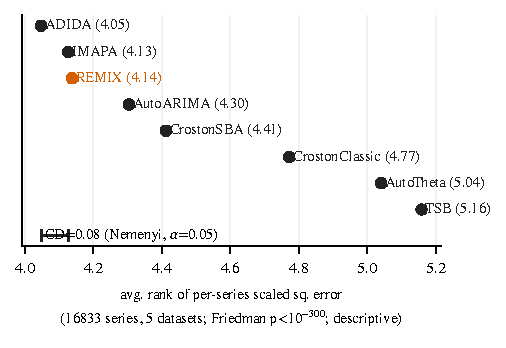
\includegraphics[width=0.93\linewidth]{figs/cd_diagram.pdf}
\caption{Average ranks of per-series scaled squared errors over the
16{,}833 series with complete saved row-level point predictions across
the five panels. The critical-difference bar is shown only for scale:
series, rather than datasets, are the blocks, so this is descriptive and
not a valid Friedman--Nemenyi test.}
\label{fig:cd}
\end{figure}

\subsection{Selection objective and efficiency}
\label{sec:criterion}\label{sec:efficiency}

The selector is not mathematically tied to pinball loss; it scores the
criterion supplied on the chronological validation tail. We use
item-averaged SPL because the target is a predictive distribution. The
best candidates are locally close, and a full cross-objective regret
matrix remains future work.

Joint selection takes $51$--$243$ seconds across the five panels,
excluding data loading, and covers 24 forecast candidates with one
deterministic EM/BIC search for the mixture on the fitting head. Final
estimation is analytic apart from low-dimensional group optimization;
selection and point prediction are deterministic, while probabilistic
bootstrap averaging uses the released fixed seed.

\subsection{Measured cost of every method}
\label{app:efficiency}

Table~\ref{tab:efficiency} reports instrumented wall-clock for every
method of Table~\ref{tab:prob} on Carparts (2{,}509 series), measured on
one CPU workstation in a single session with configurations unchanged.
The \EBB{} row includes its complete 24-candidate joint selection in
addition to the final fit ($B{=}20$) and five-quantile prediction; the
TSB-tuned row likewise includes its 25-candidate selection. No method
uses a GPU. Figure~\ref{fig:cost-accuracy} plots cost against mean SPL.

On the daily panels the official TweedieGP implementation was run in full
under the authors' released defaults (sparse variational GP with 200
inducing points and log-spaced initialization for series longer than 200
observations, all training points otherwise; Adam with learning rate
$0.1$; 50{,}000 predictive samples; median-demand scaling; restart on
numerical failure) and the authors' daily period. Online Retail
(3{,}649 series) completed with no failed fits at a per-series median of
$5.1$\,s; M5 (5{,}000 series, 1{,}294 training observations) completed
with no failed fits at a per-series median of $17.3$\,s, of which roughly
half is the 50{,}000-sample predictive draw over the 647-step external
span (the original protocol forecasts 28 steps), a protocol difference
rather than a method cost. Two caveats govern every timing in
Table~\ref{tab:efficiency}. First, all rows were measured on one machine
in one session, and absolute values are not comparable across platforms.
Second, \citet{damato2025} report $0.24$\,s per Carparts series on an M3
MacBook Pro; on our machine the released defaults give $1.89$\,s (single
thread, median of twelve series) and the paper-stated budget of 100
iterations gives $0.97$\,s, because the released code doubles the
iteration cap for Tweedie likelihoods on series with at most 500
observations.

\begin{table*}[t]
\centering
\caption{Instrumented wall-clock on Carparts, one machine, one session.
``Sel.''\ marks totals that include the method's own hyperparameter or
candidate selection. AutoARIMA/AutoTheta share one StatsForecast call
(split across the two); the five conformal wrappers share one
residual-pool fit (split across the five). Rows below the rule are
recorded from prior run metadata rather than re-timed: DeepState is a
full-panel GluonTS/MXNet run, Chronos-Bolt is zero-shot inference on a
500-series subsample, and DRP is a 500-series Online Retail subsample
(no Carparts run exists). All rows are CPU-only.}
\label{tab:efficiency}
\small
\setlength{\tabcolsep}{4.5pt}
\begin{tabular}{lrrccl}
\toprule
Method & Total (s) & s/series & Sel. & Runtime & Bit-repr.\\
\midrule
\EBB{} & 46.7 & 0.019 & yes & Python & Yes\\
TSB-tuned & 3.8 & 0.002 & yes & Python & No\\
CP wrappers (each) & 13.3 & 0.005 & no & Python & No\\
Tweedie-GLM & 37.3 & 0.015 & no & Python & No\\
iETS & 55.3 & 0.022 & no & R & No\\
AutoARIMA & 56.2 & 0.022 & no & Python & No\\
AutoTheta & 56.2 & 0.022 & no & Python & No\\
TweedieGP (12 workers) & 302.1 & 0.120 & no & Python/torch & No\\
\midrule
DeepState & 192.0 & 0.077 & no & Python/MXNet & No\\
Chronos-Bolt-small & 8.3 & 0.017 & no & Python/torch & No\\
DRP (Deep Renewal) & 1200.0 & 2.400 & no & Python/MXNet & No\\
\bottomrule
\end{tabular}
\end{table*}

\begin{table*}[t]
\centering
\caption{Walk-forward wall-clock per method and panel (seconds unless
marked in hours), covering every block of the protocol of
Table~\ref{tab:wfprob}: initialization, all per-block refits or updates,
and prediction. StatsForecast, conformal, and ACI rows run
single-process; TweedieGP runs its released code with twelve worker
processes; \EBB{} runs on one core and includes its initialization.
AutoARIMA and AutoTheta share one call. $^{\dagger}$Projected from the
measured $7{,}618$\,s full fit on the 5{,}000-series M5 sample at the
Online Retail cadence of one refit per four blocks ($24$ refits); at one
refit per block the projection is about $197$\,h. Neither was run.}
\label{tab:wfcost}
\small
\setlength{\tabcolsep}{5pt}
\begin{tabular}{lrrrrr}
\toprule
Method & Online Retail & Carparts & Auto & RAF & M5\\
\midrule
AutoARIMA & 1169 & 1.1\,h & 763 & 2.7\,h & ---\\
AutoTheta & 1169 & 1.1\,h & 763 & 2.7\,h & ---\\
iETS & 1795 & 270 & 213 & 1254 & ---\\
CP-ADIDA & --- & 9.6 & 4.4 & 38.0 & 465\\
ACI-ADIDA & 126 & 7.4 & 8.9 & 27.3 & 581\\
TweedieGP & 1.7\,h & 2686 & 2139 & 2.4\,h & $\approx$51\,h$^{\dagger}$\\
\midrule
\EBB{} & 22.4 & 3.4 & 3.6 & 13.5 & 36.6\\
ACI-\EBB{} & 52.3 & 4.2 & 4.8 & 13.3 & 217\\
\EBB{} (rule) & 22.4 & 3.4 & 4.8 & 13.5 & 217\\
\bottomrule
\end{tabular}
\end{table*}

\begin{figure}[t]
\centering
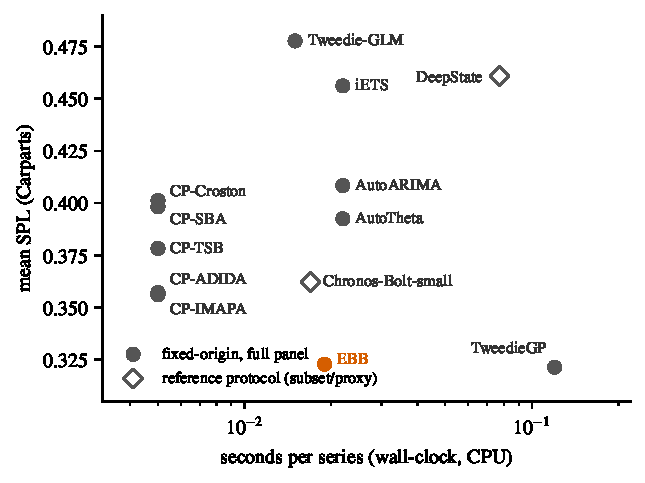
\includegraphics[width=0.95\linewidth]{figs/fig11_cost_accuracy_carparts.pdf}
\caption{Wall-clock cost per series against mean SPL on Carparts.
Filled circles are fixed-origin full-panel runs from
Table~\ref{tab:efficiency}; open diamonds are the reference points with
subset or proxy protocols. All methods run on CPU.}
\label{fig:cost-accuracy}
\end{figure}

\subsection{Controlled-study diagnostics}
\label{app:simulation-details}

In the length sweep used to isolate credibility leverage, the generator
holds $K=2$, 500 items per group, occurrence probabilities $0.05$ and
$0.80$, log-size centers three units apart, and $w=1$. The true
partition's pinball advantage falls monotonically from $1.53\%$ at
$T=12$ (median 4.5 positives per item) to $0.01\%$ at $T=400$ (median
154), with NLL, Brier, and log-size MSE following the same direction.
Across the main grid, the RMSE of $\hat\tau_g^2$ approximately doubles
as $w$ falls from $1.00$ to $0.90$ ($0.037\to0.144$ at $T=120$ and
$0.074\to0.149$ at $T=30$), directly measuring the resolution cost in
Proposition~\ref{prop:twosided}.

The generator centers the groups symmetrically around a fixed grand mean
so that increasing separation does not change total demand scale, and
every arm is evaluated through the same hurdle-lognormal predictive
representation under both likelihood-based proper scores and point
metrics. A four-arm ladder---single pool, true labels with estimated
hyperparameters, true labels with true hyperparameters, and the true
conditional law---checks the implementation; the true conditional law is
best on every metric in every cell.

\paragraph{Separation axis.} The grid above pools the three separations
$\{0.5,1,2\}$ of the original sweep, and the length sweep uses a single
separation of three; the envelope of Figure~\ref{fig:refinement-leverage}
therefore mixes separations. To resolve them we rerun the same generator
on a pre-registered grid: separation $\in\{0,0.25,0.5,1,2,3\}$ log-units
between adjacent group centers, $w\in\{1,0.95,0.90\}$, $T\in\{30,120\}$,
nine paired replicates per cell (seed 20260913), four groups of sixty
items, $\tau^2=0.15$, $\sigma^2=1$, occurrence spread in logit scaled
with the size separation as $0.8\min(\mathrm{sep},1)$ so that zero
separation removes structure from both blocks (a first pass held it fixed
at $0.8$; it is archived and superseded). Each cell records the true partition's paired pinball gain over a
single pool, the gain of the paper's mixture objective run on the same
panel, the median size-block credibility under the single pool, and the
share of item log-size variance explained by the true labels ($R^2$,
computed from the discounted item statistics so it includes sampling
noise). Two remedies for the learned mixture that already exist in the released
code are run as extra arms on the same panels: label sample-splitting
(labels from one interleaved half, hyperparameters from the other) and
credibility shrinkage of the group variance component, alone and
combined. Table~\ref{tab:sepsim} summarizes
the surface by separation and Table~\ref{tab:separation} reads it at the
real panels' coordinates. Real-panel $R^2$ uses the same statistic under
the learned mixture labels at the selected discount and under the
ADI/CV$^2$ taxonomy; we do not use the learned $\hat\tau_g^2$ as a scale
because it collapses to its floor under learned partitions
(Section~\ref{sec:leverage}). The simulation was run and summarized
before the real panels were placed.

\begin{table}[t]
\centering
\caption{Separation-resolved controlled study, averaged over the six
$(w,T)$ cells at each separation: true-label $R^2$, the true partition's
gain over a single pool, the learned mixture's gain, the same with label
sample-splitting and credibility shrinkage combined, and the median
number of components the mixture selects.}
\label{tab:sepsim}
\small
\setlength{\tabcolsep}{5pt}
\begin{tabular}{lrrrrr}
\toprule
Separation & $R^2$ & True (\%) & Learned (\%) & Learned+fix (\%) & $K$\\
\midrule
0 & 0.01 & +0.07 & -0.02 & -0.36 & 1\\
0.25 & 0.19 & +0.12 & -0.01 & -0.30 & 1\\
0.5 & 0.47 & +0.70 & -0.92 & -0.94 & 2\\
1 & 0.75 & +0.20 & -1.47 & -0.86 & 2\\
2 & 0.93 & -0.08 & -0.71 & -0.37 & 3\\
3 & 0.97 & -0.30 & -0.37 & -0.51 & 4\\
\bottomrule
\end{tabular}
\end{table}

\begin{table*}[t]
\centering
\caption{Real panels placed on the separation-resolved surface. $w$ is the
simulated discount matching the panel's selected one; $R^2$ is the
size-block separation under the learned partition and under the taxonomy,
and ``family $R^2$'' the true-label $R^2$ of the simulated family at the
panel's $\lambda^{(+)}$ ($T{=}120$). ``Room'' is the true partition's gain
interpolated along $\lambda^{(+)}$ within the matching $w$ at each length;
``sim.\ learned'' the learned mixture's gain at the same point
($T{=}120$); ``realized'' the panel's internal refinement gain
(Figure~\ref{fig:refinement-leverage}).}
\label{tab:separation}
\small
\setlength{\tabcolsep}{4.5pt}
\begin{tabular}{lrrrrrrrrr}
\toprule
Panel & $w$ & $\lambda^{(+)}$ & $R^2$ learned & $R^2$ tax. & family $R^2$ & Room $T{=}30$ & Room $T{=}120$ & Sim.\ learned & Realized\\
\midrule
Online Retail & 0.95 & 0.553 & 0.44 & 0.17 & 0.63 & -0.52 & +0.63 & -0.87 & -0.05\\
M5 & 0.95 & 0.841 & 0.79 & 0.30 & 0.86 & -0.34 & -0.45 & -1.21 & +0.58\\
Auto & 1 & 0.940 & 0.82 & 0.14 & 0.72 & -0.50 & -0.33 & -0.45 & -0.31\\
Carparts & 0.9 & 0.224 & 0.68 & 0.01 & 0.55 & +2.01 & +1.73 & -0.75 & -0.08\\
RAF & 1 & 0.917 & 0.95 & 0.09 & 0.62 & -0.48 & -0.41 & -0.58 & +0.03\\
\bottomrule
\end{tabular}
\end{table*}



\subsection{Released tables and artifacts}
Complete per-dataset tables with RMSE, WRMSSE, all quantile levels,
coverage, interval widths, fixed-corner ablations, and runtimes accompany
the code release, together with the selection surfaces and per-run
diagnostics behind every table in this paper.

\subsection{Machine-readable significance output}
The complete per-series results behind Table~\ref{tab:significance} and
Table~\ref{tab:spl-significance}, including the RMSE tests and the
Holm-adjusted families, accompany the code release as machine-readable
CSV files.

\subsection{MASE}
For completeness we report MASE (per-series MAE scaled by in-sample
naive MAE), the intermittent-demand literature's traditional point
metric. It inherits the absolute-error pathology quantified in
Section~\ref{sec:main-results}: the all-zero forecast attains the best
MASE on Online Retail ($1.84$ vs.\ TSB $2.08$, \EBB{} $2.41$),
Carparts, and RAF, and zero-leaning methods (TSB, IMAPA) lead among real
forecasters. On Auto, \EBB{} ($0.889$) is second only to CrostonSBA
($0.883$). Full table in the repository
(\texttt{mase\_table.csv}). We treat MASE as descriptive, not
decision-relevant, for the same reason as MAE.

\subsection{Walk-forward artifacts}
The complete point and probabilistic results are in
Tables~\ref{tab:walkforward} and \ref{tab:wfprob}; released block-level
artifacts retain the seven-day boundaries and every per-block prediction.

\subsection{Neural baselines}
\label{app:neural}

Table~\ref{tab:neural} retains the earlier neural comparisons. Deep
Renewal Processes (DRP) \citep{turkmen2019} are architecturally close to
our occurrence--size decomposition, but the legacy subsample numbers are
indicative only: we rebuilt the Python~3.8/MXNet~1.7 environment and
launched the original code path, yet three configurations diverged to
NaN between epochs 7 and 11 and failed during prediction. DeepAR and an
RNN under prediction-only chaining reach lower MAE in one case but worse
RMSE and RMSSE at both horizons. Neural decoding and a constant
sufficient-statistic forecast are not timing-equivalent, so these rows
should not support a broad efficiency ratio.

Two newly executed reference points provide a cleaner, narrower check.
DeepState---the published Amazon ISSM successor available in GluonTS,
not a reproduction of \citet{seeger2016}---obtains mean SPL $1.0652$ on
a 1{,}000-series Online Retail subset and $0.4608$ on full Carparts.
Chronos-Bolt-small obtains $0.8448$ on an Online Retail 500-series subset,
versus $0.8342$ for \EBB{} on exactly the same subset: a small $1.3\%$
gap. Its Carparts result is only a reference point because the same-source
Monash panel appears in the Chronos data repository and potential training
contamination cannot be excluded. These subset results motivate an
efficiency, determinism, and transparency claim, not a large foundation-
model accuracy advantage.

\begin{table}[t]
\centering
\caption{Neural comparisons on Online Retail. Top: probabilistic
(unscaled pinball, 500-series subsample, fixed protocol). Bottom: point
metrics under prediction-only chaining at two horizons.}
\label{tab:neural}
\small
\setlength{\tabcolsep}{4pt}
\begin{tabular}{lcccccc}
\toprule
 & q10 & q25 & q50 & q75 & q90 & Time\\
\midrule
DeepRenewal & 0.358 & 0.895 & 1.790 & 2.684 & 2.941 & $\sim$20\,min\\
Hierarchical EB & 0.387 & 0.914 & 1.772 & 2.390 & 2.186 & 1\,s\\
\midrule
 & \multicolumn{2}{c}{MAE} & \multicolumn{2}{c}{RMSE} & \multicolumn{2}{c}{RMSSE}\\
 & $h{=}10$ & $h{=}100$ & $h{=}10$ & $h{=}100$ & $h{=}10$ & $h{=}100$\\
\midrule
RNN & 3.257 & 3.132 & 11.938 & 12.538 & 0.875 & 8.197\\
DeepAR & 6.245 & 7.288 & 17.221 & 18.623 & 7.151 & 9.986\\
Hierarchical EB & 4.639 & 4.495 & 11.284 & 11.733 & 0.855 & 8.170\\
\bottomrule
\end{tabular}
\end{table}

\subsection{Far-tail quantiles on the sparsest panels}
\label{app:fartail}

Scaled pinball at $q\in\{0.95,0.975,0.99\}$ on the two panels where the
standard levels discriminate weakly, under the identical fixed protocol
(\EBB{} raw, $B{=}20$; iETS not re-run at these levels). The zero
forecast's scaled pinball is \emph{linear} in $q$ (its pinball at level
$q$ is $q\,\E[y/\mathrm{scale}]$), so the far tail is exactly where its
apparent advantage must collapse; the question the table answers is who
inherits the lead.

\begin{table}[h]
\centering
\small
\setlength{\tabcolsep}{3.6pt}
\begin{tabular}{lccc@{\hspace{10pt}}ccc}
\toprule
 & \multicolumn{3}{c}{Carparts} & \multicolumn{3}{c}{RAF}\\
\cmidrule(lr){2-4}\cmidrule(lr){5-7}
Model & q95 & q97.5 & q99 & q95 & q97.5 & q99\\
\midrule
CP-Croston & 0.413 & 0.290 & 0.168 & 0.488 & 0.537 & 0.526\\
CP-SBA & 0.412 & 0.290 & 0.168 & 0.489 & 0.542 & 0.529\\
CP-TSB & 0.374 & 0.263 & 0.160 & 0.506 & 0.601 & 0.552\\
CP-ADIDA & 0.384 & 0.275 & 0.159 & 0.493 & 0.579 & 0.557\\
CP-IMAPA & 0.378 & 0.270 & 0.156 & 0.493 & 0.581 & 0.564\\
AutoARIMA & 0.385 & 0.332 & 0.301 & \best{0.460} & 0.395 & 0.356\\
AutoTheta & 0.367 & 0.316 & 0.285 & 0.464 & 0.399 & 0.359\\
Tweedie-GLM & 0.581 & 0.445 & 0.305 & 0.497 & 0.439 & 0.367\\
TweedieGP & \best{0.355} & \best{0.222} & \best{0.128} & 0.462 & \best{0.352} & \secondbest{0.247}\\
\midrule
Zero & 0.710 & 0.729 & 0.740 & 0.507 & 0.520 & 0.529\\
\midrule
\EBB{} & \secondbest{0.365} & \secondbest{0.251} & \secondbest{0.144} & \secondbest{0.461} & \secondbest{0.364} & \best{0.246}\\
\bottomrule
\end{tabular}
\end{table}

Three readings follow. First, \textbf{the saturation breaks as expected}:
on RAF the zero forecast, marginally ahead at $q\le0.9$, falls behind
every intensity-bearing method from $q{=}0.95$ on, and on Carparts it is
last by a factor of two. Second, \textbf{tail leadership is
model-specific}: official TweedieGP wins all three Carparts cells, while
\EBB{} is second in all three; on RAF, AutoARIMA wins q95, TweedieGP
wins q97.5, and \EBB{} wins q99 by a near tie. Third, this table
deliberately narrows the claim: \EBB{}'s most consistent advantage is
aggregate SPL, not universal extreme-quantile dominance. The conformal
wrappers still deteriorate in the RAF far tail, where their per-level
calibration information is sparse.

\subsection{Full-posterior inference on the same hierarchy}
\label{app:mcmc}

To separate the inference method from the model, we paired plug-in EB
with a full-posterior sampler at each discount. Each pair uses the same
single global pool, shared size-variance specification, discounted
sufficient statistics, seed-controlled 500-series Online Retail subsample,
evaluation span, and scoring code. The sampler uses
Metropolis-within-Gibbs for the Beta hyperparameters, four deterministic
chains of 4{,}000 sweeps, 2{,}000 burn-in iterations, and thinning by four.
Both a stationary version ($w{=}1$) and a power-prior discounted version
($w{=}0.98$) are tested. The richer \EBB{} arm runs its joint
selection separately on this subsample and is
reported only as context, not as an inference-method contrast.

\begin{table}[h]
\centering
\small
\begin{tabular}{lccccc}
\toprule
 & SPL mean & SPL q90 & MAE & RMSSE & sec.\\
\midrule
\EBB{} (incl.\ selection) & 0.7942 & 1.3682 & 5.6259 & 4.6712 & 86.4\\
EB global, $w{=}1$ & 0.7919 & 1.3588 & 5.5504 & 4.6684 & 0.2\\
Gibbs global, $w{=}1$ & 0.7919 & 1.3590 & 5.5890 & 4.6696 & 2.7\\
EB global, $w{=}0.98$ & 0.7935 & 1.3658 & 5.4774 & 4.6694 & 0.2\\
Gibbs global, $w{=}0.98$ & 0.7937 & 1.3665 & 5.5549 & 4.6734 & 2.7\\
\bottomrule
\end{tabular}
\end{table}

Two readings. First, \emph{the empirical-Bayes approximation is not a
distributional-accuracy bottleneck}: paired full-posterior inference changes
mean SPL by $0.007\%/0.019\%$, q90 SPL by $0.018\%/0.048\%$, and RMSSE by
$0.025\%/0.085\%$ at $w=1/0.98$. MAE is somewhat more sensitive but still
changes only $0.70\%/1.42\%$. Second, forgetting helps MAE under both
inference methods, so that finding is not an artifact of the EB plug-in.
The maximum split-$\widehat R$ across $(\alpha,\beta,\mu_0,\tau^2,\sigma^2)$
is $1.0021$, and the minimum effective sample size is $819$ of 2{,}000
retained draws.
What this experiment does \emph{not} measure: the richer external
state-space samplers
\citep{chapados2014,seeger2016} remain unrun (Limitations, item~6); this
conjugate single-pool Gibbs is far cheaper than those models and is a
control for the inference method, not a stand-in for them. The plug-in
EB path retains bit-reproducibility and requires no convergence
diagnostics, but at this scale raw speed does not separate the two.

\subsection{Datasets}\label{app:datasets}
Online Retail: UCI 352; returns/zero-price removed, 99.5\% quantity cap,
daily aggregation densified with zeros. M5: Kaggle M5-Accuracy;
seed-controlled 5{,}000-series sample. Both M5 protocols use a two-thirds
initialization split; the learned mixture is selected at $w=0.95$ on all
three audited seeds. Auto/RAF: gluon-ts
\texttt{intermittent-datasets} branch. Carparts: Zenodo 4656022, series
without missing values and with at least one zero (2{,}509). Monthly
panels use the last-$h$ holdout of \citet{damato2025}.



\end{document}
